%%%%%%%%%%%%%%%%%%%%%%%%%%%%%%%%%%%%%%%%%%%%%%%%%%%%%%%%%%%%%%%%%%%%%%%%%%%%%%%%
\subsection{Πειραματική διαδικασία}
\label{subsection:02_03_04:01}


Προκειμένου να ελεγχθεί η αποτελεσματικότητα της προτεινόμενης μεθόδου ??
πραγματοποιούμε πειράματα σε διαφορετικά---δομημένα και αδόμητα---περιβάλλοντα,
και υπό διαφορετικές αναλύσεις των χαρτών τους. Προκειμένου να ελεγχθεί η
ευρωστία της προτεινόμενης μεθόδου απέναντι στην επίδραση διαταραχών, εκτελούμε
την πειραματική διαδικασία έναντι επιπέδων θορύβων που φέρουν διαθέσιμοι
εμπορικοί αισθητήρες. Το ρομπότ που χρησιμοποιήθηκε σε όλες τις προσομοιώσεις
ήταν ένα Turtlebot v.$2$, εξοπλισμένο με έναν αισθητήρα lidar μέγιστου
ακτινικού εύρους $10.0$ μέτρων, ο οποίος αναφέρει $N_s=720$ μετρήσεις δύο
διαστάσεων, σε γωνιακό εύρος $360$ μοιρών. Η μέγιστη ανιχνευόμενη ακτινική
απόσταση ορίστηκε σε αυτή την τιμή προκειμένου να περιορίζεται ο όγκος των
πληροφοριών που είναι διαθέσιμες σε κάθε μέθοδο ευθυγράμμισης, ώστε να ελεγχθεί
ταυτόχρονα η ευρωστία τους έναντι της απουσίας πληροφοριών, πέραν αυτής που
αφορά στην αβεβαιότητα τους.  Για να ελεγχθεί η επίδοση της προτεινόμενης
μεθόδου σε πραγματικές συνθήκες, χρησιμοποιήθηκε ο αισθητήρας YDLIDAR TG30. Η
μέγιστη ανιχνευόμενη ακτινική απόστασή του είναι $30.0$ m, και ο αριθμός των
εκπεμπόμενων ακτίνων είναι $N_s = 2019$ \cite{ydlidar}. Παράλληλα, η επίδοση της
προτεινόμενης μέθοδου PGL-FMIC αντιπαραβάλλεται με τον αλγόριθμο PLICP σε μια
προσπάθεια να καταγραφούν τα συγκριτικά πλεονεκτήματα και μειονεκτήματα των δύο
μεθόδων. Ο τρόπος με τον οποίο ο PLICP μπορεί να χρησιμοποιηθεί για την επίλυση
του προβλήματος της εκτίμησης της στάσης ενός ρομπότ του πεδίου εφαρμογής βάσει
καθολικής αβεβαιότητος περιγράφηκε στην ενότητα \ref{subsection:02_02_05:02}.

Και οι δύο αλγόριθμοι δοκιμάστηκαν σε πέντε προσομοιωμένα περιβάλλοντα, τα οποία
ονομάζονται CORRIDOR, HOME, WAREHOUSE, WILLOWGARAGE, και LANDFILL, για συνολικά
$38$ στάσεις ρομπότ, και για τρία επίπεδα θορύβου του αισθητήρα απόστασης. Ο
θόρυβος που διαταράσσει τις μετρήσεις του είναι κανονικά κατανεμημένος με
τυπική απόκλιση $d \in \mathcal{D} = \{0.01, 0.02, 0.05\}$ m και μηδενική μέση
τιμή. Οι αποστάσεις των εικονικών σαρώσεων διαταράσσονται αναλογικά με την
παραποίηση του περιβάλλοντος στο οποίο αντιστοιχεί ο χάρτης. Οι χάρτες των
περιβαλλόντων CORRIDOR ($\bm{M}_C$), HOME ($\bm{M}_H$), WAREHOUSE ($\bm{M}_W$),
και LANDFILL ($\bm{M}_L$) κατασκευάστηκαν με το ίδιο ρομπότ, του οποίου οι
μετρήσεις διαταράσσονται από θόρυβο κανονικά κατανεμημένο, με μηδενική μέση
τιμή, και τυπική απόκλιση $d = 0.01$ m. Το περιβάλλον από το οποίο
δημιουργήθηκε ο χάρτης $\bm{M}_L$ κατασκευάστηκε από μοντέλα του συνόλου
δεδομένων \texttt{3DGEMS} \cite{Rasouli2017}, ενώ ο χάρτης $\bm{M}_G$ λήφθηκε από
το \cite{willow_map}.  Οι δύο αλγόριθμοι δοκιμάστηκαν επίσης σε ένα πραγματικό
περιβάλλον, σε $11$ πραγματικές στάσεις του ρομπότ. Τα πειράματα σε πραγματικές
συνθήκες πραγματοποιήθηκαν στο Εργαστήριο Αρχιτεκτονικής Συστημάτων και
Υπολογιστών (CSAL) του Αριστοτελείου Πανεπιστημίου Θεσσαλονίκης (ΑΠΘ). Ο
χάρτης του CSAL $\bm{M}_A$ κατασκευάστηκε με τη χρήση ενός Turtlebot v.$2$,
(εικόνα \ref{img:tb_yd}).

Για τον προσδιορισμό κάθε στάσης του ρομπότ κάθε προσομοίωση πραγματοποιήθηκε
$N = 100$ φορές για κάθε αλγόριθμο για λόγους αξιοπιστίας των συμπερασμάτων.  Ο
συνολικός αριθμός των προσομοιώσεων που πραγματοποιήθηκαν για κάθε μέθοδο ήταν
επομένως $ 38 \times 100 \times 3 \sim \mathcal{O}(4)$.  Για τον προσδιορισμό
κάθε στάσης του ρομπότ στο πραγματικό περιβάλον κάθε πείραμα πραγματοποιήθηκε
$N = 5$ φορές.

Τα πέντε προσομοιωμένα περιβάλλοντα απεικονίζονται στα σχήματα
\ref{fig:02_03_04:map_corridor}-\ref{fig:02_03_04:map_landfill}. To σχήμα
\ref{fig:map_corridor_simulation} απεικονίζει ένα απλό και σχεδόν συμμετρικό
περιβάλλον που χρησιμοποιείται για προκαταρκτική αξιολόγηση και σκοπούς
διάκρισης στάσεων λόγω της συμμετρίας του. Το σχήμα \ref{fig:02_03_04:map_home}
απεικονίζει ένα τυπικό οικιακό ή εμπορικό χώρο γεμάτο με καρέκλες, τραπέζια,
στήλες και ορθογώνια έπιπλα. Το σχήμα \ref{fig:02_03_04:map_warehouse}
απεικονίζει έναν τυπικό περιβάλλον αποθήκης, με μεγάλους ανοιχτούς χώρους στους
οποίους δοκιμάζεται η ικανότητα των μεθόδων να ανταπεξέλθουν σε ελλειπείς
πληροφορίες. Στο σχήμα \ref{fig:02_03_04:map_willowgarage} απεικονίζεται ένα
μεγάλο συγκρότημα που ομοιάζει με σύμπλεγμα γραφείων, όπου οι μέθοδοι
αξιολογούνται περισσότερο προσεκτικά ως προς την ικανότητά τους να επιλύουν
ασάφειες στάσης. Το σχήμα \ref{fig:map_landfill_simulation} απεικονίζει ένα μη
δομημένο περιβάλλον παρόμοιο με αυτό μίας χωματερής, το οποίιο χρησιμοποιείται
για να διαπιστωθεί η εγκυρότητα του ισχυρισμού ότι η επίδοση του PGL-FMIC δεν
κάνει διάκριση μεταξύ δομημένων και μη περιβαλλόντων. Οι χάρτες των δύο
τελευταίων περιβαλλόντων (WILLOWGARAGE και LANDFILL) έχουν ανάλυση
$0.05\times0.05$ m$^2$, ενώ εκείνοι των άλλων τριών $0.01\times0.01$ m$^2$. Ο
χάρτης του εργαστηρίου CSAL απεικονίζεται στο σχήμα
\ref{fig:02_03_04:map_csal}, και η ανάλυση του είναι $0.05\times0.05$ m$^2$.

\begin{figure}
  \begin{subfigure}{0.5\linewidth}
    % GNUPLOT: LaTeX picture with Postscript
\begingroup
  \makeatletter
  \providecommand\color[2][]{%
    \GenericError{(gnuplot) \space\space\space\@spaces}{%
      Package color not loaded in conjunction with
      terminal option `colourtext'%
    }{See the gnuplot documentation for explanation.%
    }{Either use 'blacktext' in gnuplot or load the package
      color.sty in LaTeX.}%
    \renewcommand\color[2][]{}%
  }%
  \providecommand\includegraphics[2][]{%
    \GenericError{(gnuplot) \space\space\space\@spaces}{%
      Package graphicx or graphics not loaded%
    }{See the gnuplot documentation for explanation.%
    }{The gnuplot epslatex terminal needs graphicx.sty or graphics.sty.}%
    \renewcommand\includegraphics[2][]{}%
  }%
  \providecommand\rotatebox[2]{#2}%
  \@ifundefined{ifGPcolor}{%
    \newif\ifGPcolor
    \GPcolorfalse
  }{}%
  \@ifundefined{ifGPblacktext}{%
    \newif\ifGPblacktext
    \GPblacktexttrue
  }{}%
  % define a \g@addto@macro without @ in the name:
  \let\gplgaddtomacro\g@addto@macro
  % define empty templates for all commands taking text:
  \gdef\gplfronttext{}%
  \gdef\gplfronttext{}%
  \makeatother
  \ifGPblacktext
    % no textcolor at all
    \def\colorrgb#1{}%
    \def\colorgray#1{}%
  \else
    % gray or color?
    \ifGPcolor
      \def\colorrgb#1{\color[rgb]{#1}}%
      \def\colorgray#1{\color[gray]{#1}}%
      \expandafter\def\csname LTw\endcsname{\color{white}}%
      \expandafter\def\csname LTb\endcsname{\color{black}}%
      \expandafter\def\csname LTa\endcsname{\color{black}}%
      \expandafter\def\csname LT0\endcsname{\color[rgb]{1,0,0}}%
      \expandafter\def\csname LT1\endcsname{\color[rgb]{0,1,0}}%
      \expandafter\def\csname LT2\endcsname{\color[rgb]{0,0,1}}%
      \expandafter\def\csname LT3\endcsname{\color[rgb]{1,0,1}}%
      \expandafter\def\csname LT4\endcsname{\color[rgb]{0,1,1}}%
      \expandafter\def\csname LT5\endcsname{\color[rgb]{1,1,0}}%
      \expandafter\def\csname LT6\endcsname{\color[rgb]{0,0,0}}%
      \expandafter\def\csname LT7\endcsname{\color[rgb]{1,0.3,0}}%
      \expandafter\def\csname LT8\endcsname{\color[rgb]{0.5,0.5,0.5}}%
    \else
      % gray
      \def\colorrgb#1{\color{black}}%
      \def\colorgray#1{\color[gray]{#1}}%
      \expandafter\def\csname LTw\endcsname{\color{white}}%
      \expandafter\def\csname LTb\endcsname{\color{black}}%
      \expandafter\def\csname LTa\endcsname{\color{black}}%
      \expandafter\def\csname LT0\endcsname{\color{black}}%
      \expandafter\def\csname LT1\endcsname{\color{black}}%
      \expandafter\def\csname LT2\endcsname{\color{black}}%
      \expandafter\def\csname LT3\endcsname{\color{black}}%
      \expandafter\def\csname LT4\endcsname{\color{black}}%
      \expandafter\def\csname LT5\endcsname{\color{black}}%
      \expandafter\def\csname LT6\endcsname{\color{black}}%
      \expandafter\def\csname LT7\endcsname{\color{black}}%
      \expandafter\def\csname LT8\endcsname{\color{black}}%
    \fi
  \fi
  \setlength{\unitlength}{0.0500bp}%
  \begin{picture}(4000.00,4000.00)%
    \gplgaddtomacro\gplfronttext{%
      \colorrgb{0.00,0.00,0.00}%
      \put(388,877){\makebox(0,0)[r]{\strut{}4}}%
      \colorrgb{0.00,0.00,0.00}%
      \put(388,1354){\makebox(0,0)[r]{\strut{}6}}%
      \colorrgb{0.00,0.00,0.00}%
      \put(388,1831){\makebox(0,0)[r]{\strut{}8}}%
      \colorrgb{0.00,0.00,0.00}%
      \put(388,2307){\makebox(0,0)[r]{\strut{}10}}%
      \colorrgb{0.00,0.00,0.00}%
      \put(388,2784){\makebox(0,0)[r]{\strut{}12}}%
      \colorrgb{0.00,0.00,0.00}%
      \put(388,3261){\makebox(0,0)[r]{\strut{}14}}%
      \colorrgb{0.00,0.00,0.00}%
      \put(520,419){\makebox(0,0){\strut{}2}}%
      \colorrgb{0.00,0.00,0.00}%
      \put(997,419){\makebox(0,0){\strut{}4}}%
      \colorrgb{0.00,0.00,0.00}%
      \put(1474,419){\makebox(0,0){\strut{}6}}%
      \colorrgb{0.00,0.00,0.00}%
      \put(1950,419){\makebox(0,0){\strut{}8}}%
      \colorrgb{0.00,0.00,0.00}%
      \put(2427,419){\makebox(0,0){\strut{}10}}%
      \colorrgb{0.00,0.00,0.00}%
      \put(2904,419){\makebox(0,0){\strut{}12}}%
      \colorrgb{0.00,0.00,0.00}%
      \put(3381,419){\makebox(0,0){\strut{}14}}%
      \colorrgb{0.00,0.00,0.00}%
      \put(-118,2069){\rotatebox{90}{\makebox(0,0){\strut{}$y$ [m]}}}%
      \colorrgb{0.00,0.00,0.00}%
      \put(2069,89){\makebox(0,0){\strut{}$x$ [m]}}%
    }%
    \gplgaddtomacro\gplfronttext{%
    }%
    \put(0,0){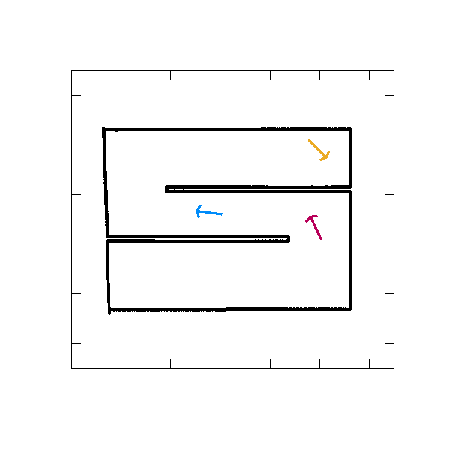
\includegraphics{./figures/parts/02/chapters/03/sections/04/map_corridor}}%
    \gplfronttext
  \end{picture}%
\endgroup

    %\caption{\small Ο χάρτης $\bm{M}_C$ του περιβάλλοντος CORRIDOR}
    \label{fig:02_03_04:map_corridor}
  \end{subfigure}%
  \begin{subfigure}{0.5\linewidth}
    % GNUPLOT: LaTeX picture with Postscript
\begingroup
  \makeatletter
  \providecommand\color[2][]{%
    \GenericError{(gnuplot) \space\space\space\@spaces}{%
      Package color not loaded in conjunction with
      terminal option `colourtext'%
    }{See the gnuplot documentation for explanation.%
    }{Either use 'blacktext' in gnuplot or load the package
      color.sty in LaTeX.}%
    \renewcommand\color[2][]{}%
  }%
  \providecommand\includegraphics[2][]{%
    \GenericError{(gnuplot) \space\space\space\@spaces}{%
      Package graphicx or graphics not loaded%
    }{See the gnuplot documentation for explanation.%
    }{The gnuplot epslatex terminal needs graphicx.sty or graphics.sty.}%
    \renewcommand\includegraphics[2][]{}%
  }%
  \providecommand\rotatebox[2]{#2}%
  \@ifundefined{ifGPcolor}{%
    \newif\ifGPcolor
    \GPcolorfalse
  }{}%
  \@ifundefined{ifGPblacktext}{%
    \newif\ifGPblacktext
    \GPblacktexttrue
  }{}%
  % define a \g@addto@macro without @ in the name:
  \let\gplgaddtomacro\g@addto@macro
  % define empty templates for all commands taking text:
  \gdef\gplfronttext{}%
  \gdef\gplfronttext{}%
  \makeatother
  \ifGPblacktext
    % no textcolor at all
    \def\colorrgb#1{}%
    \def\colorgray#1{}%
  \else
    % gray or color?
    \ifGPcolor
      \def\colorrgb#1{\color[rgb]{#1}}%
      \def\colorgray#1{\color[gray]{#1}}%
      \expandafter\def\csname LTw\endcsname{\color{white}}%
      \expandafter\def\csname LTb\endcsname{\color{black}}%
      \expandafter\def\csname LTa\endcsname{\color{black}}%
      \expandafter\def\csname LT0\endcsname{\color[rgb]{1,0,0}}%
      \expandafter\def\csname LT1\endcsname{\color[rgb]{0,1,0}}%
      \expandafter\def\csname LT2\endcsname{\color[rgb]{0,0,1}}%
      \expandafter\def\csname LT3\endcsname{\color[rgb]{1,0,1}}%
      \expandafter\def\csname LT4\endcsname{\color[rgb]{0,1,1}}%
      \expandafter\def\csname LT5\endcsname{\color[rgb]{1,1,0}}%
      \expandafter\def\csname LT6\endcsname{\color[rgb]{0,0,0}}%
      \expandafter\def\csname LT7\endcsname{\color[rgb]{1,0.3,0}}%
      \expandafter\def\csname LT8\endcsname{\color[rgb]{0.5,0.5,0.5}}%
    \else
      % gray
      \def\colorrgb#1{\color{black}}%
      \def\colorgray#1{\color[gray]{#1}}%
      \expandafter\def\csname LTw\endcsname{\color{white}}%
      \expandafter\def\csname LTb\endcsname{\color{black}}%
      \expandafter\def\csname LTa\endcsname{\color{black}}%
      \expandafter\def\csname LT0\endcsname{\color{black}}%
      \expandafter\def\csname LT1\endcsname{\color{black}}%
      \expandafter\def\csname LT2\endcsname{\color{black}}%
      \expandafter\def\csname LT3\endcsname{\color{black}}%
      \expandafter\def\csname LT4\endcsname{\color{black}}%
      \expandafter\def\csname LT5\endcsname{\color{black}}%
      \expandafter\def\csname LT6\endcsname{\color{black}}%
      \expandafter\def\csname LT7\endcsname{\color{black}}%
      \expandafter\def\csname LT8\endcsname{\color{black}}%
    \fi
  \fi
  \setlength{\unitlength}{0.0500bp}%
  \begin{picture}(4000.00,4000.00)%
    \gplgaddtomacro\gplfronttext{%
      \colorrgb{0.00,0.00,0.00}%
      \put(388,900){\makebox(0,0)[r]{\strut{}5}}%
      \colorrgb{0.00,0.00,0.00}%
      \put(388,1408){\makebox(0,0)[r]{\strut{}10}}%
      \colorrgb{0.00,0.00,0.00}%
      \put(388,1917){\makebox(0,0)[r]{\strut{}15}}%
      \colorrgb{0.00,0.00,0.00}%
      \put(388,2425){\makebox(0,0)[r]{\strut{}20}}%
      \colorrgb{0.00,0.00,0.00}%
      \put(388,2933){\makebox(0,0)[r]{\strut{}25}}%
      \colorrgb{0.00,0.00,0.00}%
      \put(388,3441){\makebox(0,0)[r]{\strut{}30}}%
      \colorrgb{0.00,0.00,0.00}%
      \put(571,477){\makebox(0,0){\strut{}10}}%
      \colorrgb{0.00,0.00,0.00}%
      \put(1079,477){\makebox(0,0){\strut{}15}}%
      \colorrgb{0.00,0.00,0.00}%
      \put(1587,477){\makebox(0,0){\strut{}20}}%
      \colorrgb{0.00,0.00,0.00}%
      \put(2095,477){\makebox(0,0){\strut{}25}}%
      \colorrgb{0.00,0.00,0.00}%
      \put(2603,477){\makebox(0,0){\strut{}30}}%
      \colorrgb{0.00,0.00,0.00}%
      \put(3111,477){\makebox(0,0){\strut{}35}}%
      \colorrgb{0.00,0.00,0.00}%
      \put(3619,477){\makebox(0,0){\strut{}40}}%
      \colorrgb{0.00,0.00,0.00}%
      \put(-118,2069){\rotatebox{90}{\makebox(0,0){\strut{}$y$ [m]}}}%
      \colorrgb{0.00,0.00,0.00}%
      \put(2069,147){\makebox(0,0){\strut{}$x$ [m]}}%
      \put(2000,3700){\makebox(0,0){HOME}}%
    }%
    \gplgaddtomacro\gplfronttext{%
    }%
    \put(0,0){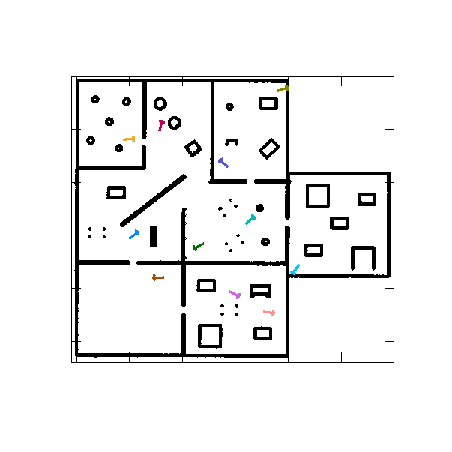
\includegraphics{./figures/parts/02/chapters/03/sections/04/map_home}}%
    \gplfronttext
  \end{picture}%
\endgroup

    %\caption{\small Ο χάρτης $\bm{M}_H$ του περιβάλλοντος HOME}
    \label{fig:02_03_04:map_home}
  \end{subfigure}\\
  \begin{subfigure}{0.5\linewidth}
    \vspace{0.5cm}
    % GNUPLOT: LaTeX picture with Postscript
\begingroup
  \makeatletter
  \providecommand\color[2][]{%
    \GenericError{(gnuplot) \space\space\space\@spaces}{%
      Package color not loaded in conjunction with
      terminal option `colourtext'%
    }{See the gnuplot documentation for explanation.%
    }{Either use 'blacktext' in gnuplot or load the package
      color.sty in LaTeX.}%
    \renewcommand\color[2][]{}%
  }%
  \providecommand\includegraphics[2][]{%
    \GenericError{(gnuplot) \space\space\space\@spaces}{%
      Package graphicx or graphics not loaded%
    }{See the gnuplot documentation for explanation.%
    }{The gnuplot epslatex terminal needs graphicx.sty or graphics.sty.}%
    \renewcommand\includegraphics[2][]{}%
  }%
  \providecommand\rotatebox[2]{#2}%
  \@ifundefined{ifGPcolor}{%
    \newif\ifGPcolor
    \GPcolorfalse
  }{}%
  \@ifundefined{ifGPblacktext}{%
    \newif\ifGPblacktext
    \GPblacktexttrue
  }{}%
  % define a \g@addto@macro without @ in the name:
  \let\gplgaddtomacro\g@addto@macro
  % define empty templates for all commands taking text:
  \gdef\gplfronttext{}%
  \gdef\gplfronttext{}%
  \makeatother
  \ifGPblacktext
    % no textcolor at all
    \def\colorrgb#1{}%
    \def\colorgray#1{}%
  \else
    % gray or color?
    \ifGPcolor
      \def\colorrgb#1{\color[rgb]{#1}}%
      \def\colorgray#1{\color[gray]{#1}}%
      \expandafter\def\csname LTw\endcsname{\color{white}}%
      \expandafter\def\csname LTb\endcsname{\color{black}}%
      \expandafter\def\csname LTa\endcsname{\color{black}}%
      \expandafter\def\csname LT0\endcsname{\color[rgb]{1,0,0}}%
      \expandafter\def\csname LT1\endcsname{\color[rgb]{0,1,0}}%
      \expandafter\def\csname LT2\endcsname{\color[rgb]{0,0,1}}%
      \expandafter\def\csname LT3\endcsname{\color[rgb]{1,0,1}}%
      \expandafter\def\csname LT4\endcsname{\color[rgb]{0,1,1}}%
      \expandafter\def\csname LT5\endcsname{\color[rgb]{1,1,0}}%
      \expandafter\def\csname LT6\endcsname{\color[rgb]{0,0,0}}%
      \expandafter\def\csname LT7\endcsname{\color[rgb]{1,0.3,0}}%
      \expandafter\def\csname LT8\endcsname{\color[rgb]{0.5,0.5,0.5}}%
    \else
      % gray
      \def\colorrgb#1{\color{black}}%
      \def\colorgray#1{\color[gray]{#1}}%
      \expandafter\def\csname LTw\endcsname{\color{white}}%
      \expandafter\def\csname LTb\endcsname{\color{black}}%
      \expandafter\def\csname LTa\endcsname{\color{black}}%
      \expandafter\def\csname LT0\endcsname{\color{black}}%
      \expandafter\def\csname LT1\endcsname{\color{black}}%
      \expandafter\def\csname LT2\endcsname{\color{black}}%
      \expandafter\def\csname LT3\endcsname{\color{black}}%
      \expandafter\def\csname LT4\endcsname{\color{black}}%
      \expandafter\def\csname LT5\endcsname{\color{black}}%
      \expandafter\def\csname LT6\endcsname{\color{black}}%
      \expandafter\def\csname LT7\endcsname{\color{black}}%
      \expandafter\def\csname LT8\endcsname{\color{black}}%
    \fi
  \fi
  \setlength{\unitlength}{0.0500bp}%
  \begin{picture}(4000.00,5000.00)%
    \gplgaddtomacro\gplfronttext{%
      \colorrgb{0.00,0.00,0.00}%
      \put(870,550){\makebox(0,0)[r]{\strut{}0}}%
      \colorrgb{0.00,0.00,0.00}%
      \put(870,1035){\makebox(0,0)[r]{\strut{}5}}%
      \colorrgb{0.00,0.00,0.00}%
      \put(870,1520){\makebox(0,0)[r]{\strut{}10}}%
      \colorrgb{0.00,0.00,0.00}%
      \put(870,2005){\makebox(0,0)[r]{\strut{}15}}%
      \colorrgb{0.00,0.00,0.00}%
      \put(870,2490){\makebox(0,0)[r]{\strut{}20}}%
      \colorrgb{0.00,0.00,0.00}%
      \put(870,2975){\makebox(0,0)[r]{\strut{}25}}%
      \colorrgb{0.00,0.00,0.00}%
      \put(870,3460){\makebox(0,0)[r]{\strut{}30}}%
      \colorrgb{0.00,0.00,0.00}%
      \put(870,3945){\makebox(0,0)[r]{\strut{}35}}%
      \colorrgb{0.00,0.00,0.00}%
      \put(870,4430){\makebox(0,0)[r]{\strut{}40}}%
      \colorrgb{0.00,0.00,0.00}%
      \put(1002,330){\makebox(0,0){\strut{}0}}%
      \colorrgb{0.00,0.00,0.00}%
      \put(1487,330){\makebox(0,0){\strut{}5}}%
      \colorrgb{0.00,0.00,0.00}%
      \put(1972,330){\makebox(0,0){\strut{}10}}%
      \colorrgb{0.00,0.00,0.00}%
      \put(2457,330){\makebox(0,0){\strut{}15}}%
      \colorrgb{0.00,0.00,0.00}%
      \put(2942,330){\makebox(0,0){\strut{}20}}%
      \colorrgb{0.00,0.00,0.00}%
      \put(364,2587){\rotatebox{90}{\makebox(0,0){\strut{}$y$ [m]}}}%
      \colorrgb{0.00,0.00,0.00}%
      \put(2069,0){\makebox(0,0){\strut{}$x$ [m]}}%
    }%
    \gplgaddtomacro\gplfronttext{%
    }%
    \put(0,0){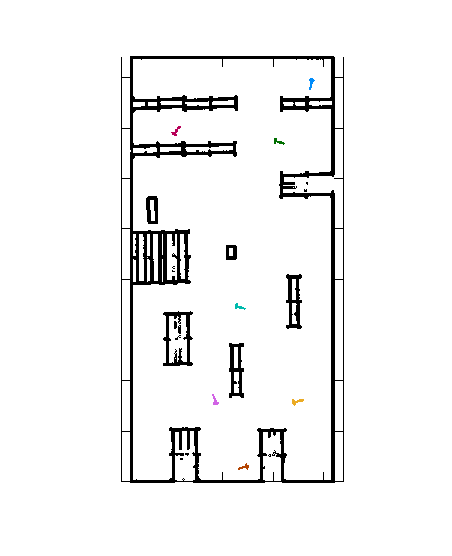
\includegraphics{./figures/parts/02/chapters/03/sections/04/map_warehouse}}%
    \gplfronttext
  \end{picture}%
\endgroup

    %\caption{\small Ο χάρτης $\bm{M}_W$ του περιβάλλοντος WAREHOUSE}
    \label{fig:02_03_04:map_warehouse}
  \end{subfigure}
  \begin{subfigure}{0.5\linewidth}
    % GNUPLOT: LaTeX picture with Postscript
\begingroup
  \makeatletter
  \providecommand\color[2][]{%
    \GenericError{(gnuplot) \space\space\space\@spaces}{%
      Package color not loaded in conjunction with
      terminal option `colourtext'%
    }{See the gnuplot documentation for explanation.%
    }{Either use 'blacktext' in gnuplot or load the package
      color.sty in LaTeX.}%
    \renewcommand\color[2][]{}%
  }%
  \providecommand\includegraphics[2][]{%
    \GenericError{(gnuplot) \space\space\space\@spaces}{%
      Package graphicx or graphics not loaded%
    }{See the gnuplot documentation for explanation.%
    }{The gnuplot epslatex terminal needs graphicx.sty or graphics.sty.}%
    \renewcommand\includegraphics[2][]{}%
  }%
  \providecommand\rotatebox[2]{#2}%
  \@ifundefined{ifGPcolor}{%
    \newif\ifGPcolor
    \GPcolorfalse
  }{}%
  \@ifundefined{ifGPblacktext}{%
    \newif\ifGPblacktext
    \GPblacktexttrue
  }{}%
  % define a \g@addto@macro without @ in the name:
  \let\gplgaddtomacro\g@addto@macro
  % define empty templates for all commands taking text:
  \gdef\gplfronttext{}%
  \gdef\gplfronttext{}%
  \makeatother
  \ifGPblacktext
    % no textcolor at all
    \def\colorrgb#1{}%
    \def\colorgray#1{}%
  \else
    % gray or color?
    \ifGPcolor
      \def\colorrgb#1{\color[rgb]{#1}}%
      \def\colorgray#1{\color[gray]{#1}}%
      \expandafter\def\csname LTw\endcsname{\color{white}}%
      \expandafter\def\csname LTb\endcsname{\color{black}}%
      \expandafter\def\csname LTa\endcsname{\color{black}}%
      \expandafter\def\csname LT0\endcsname{\color[rgb]{1,0,0}}%
      \expandafter\def\csname LT1\endcsname{\color[rgb]{0,1,0}}%
      \expandafter\def\csname LT2\endcsname{\color[rgb]{0,0,1}}%
      \expandafter\def\csname LT3\endcsname{\color[rgb]{1,0,1}}%
      \expandafter\def\csname LT4\endcsname{\color[rgb]{0,1,1}}%
      \expandafter\def\csname LT5\endcsname{\color[rgb]{1,1,0}}%
      \expandafter\def\csname LT6\endcsname{\color[rgb]{0,0,0}}%
      \expandafter\def\csname LT7\endcsname{\color[rgb]{1,0.3,0}}%
      \expandafter\def\csname LT8\endcsname{\color[rgb]{0.5,0.5,0.5}}%
    \else
      % gray
      \def\colorrgb#1{\color{black}}%
      \def\colorgray#1{\color[gray]{#1}}%
      \expandafter\def\csname LTw\endcsname{\color{white}}%
      \expandafter\def\csname LTb\endcsname{\color{black}}%
      \expandafter\def\csname LTa\endcsname{\color{black}}%
      \expandafter\def\csname LT0\endcsname{\color{black}}%
      \expandafter\def\csname LT1\endcsname{\color{black}}%
      \expandafter\def\csname LT2\endcsname{\color{black}}%
      \expandafter\def\csname LT3\endcsname{\color{black}}%
      \expandafter\def\csname LT4\endcsname{\color{black}}%
      \expandafter\def\csname LT5\endcsname{\color{black}}%
      \expandafter\def\csname LT6\endcsname{\color{black}}%
      \expandafter\def\csname LT7\endcsname{\color{black}}%
      \expandafter\def\csname LT8\endcsname{\color{black}}%
    \fi
  \fi
  \setlength{\unitlength}{0.0500bp}%
  \begin{picture}(4000.00,4000.00)%
    \gplgaddtomacro\gplfronttext{%
      \colorrgb{0.00,0.00,0.00}%
      \put(388,485){\makebox(0,0)[r]{\strut{}35}}%
      \colorrgb{0.00,0.00,0.00}%
      \put(388,829){\makebox(0,0)[r]{\strut{}40}}%
      \colorrgb{0.00,0.00,0.00}%
      \put(388,1174){\makebox(0,0)[r]{\strut{}45}}%
      \colorrgb{0.00,0.00,0.00}%
      \put(388,1518){\makebox(0,0)[r]{\strut{}50}}%
      \colorrgb{0.00,0.00,0.00}%
      \put(388,1862){\makebox(0,0)[r]{\strut{}55}}%
      \colorrgb{0.00,0.00,0.00}%
      \put(388,2207){\makebox(0,0)[r]{\strut{}60}}%
      \colorrgb{0.00,0.00,0.00}%
      \put(388,2551){\makebox(0,0)[r]{\strut{}65}}%
      \colorrgb{0.00,0.00,0.00}%
      \put(388,2895){\makebox(0,0)[r]{\strut{}70}}%
      \colorrgb{0.00,0.00,0.00}%
      \put(388,3240){\makebox(0,0)[r]{\strut{}75}}%
      \colorrgb{0.00,0.00,0.00}%
      \put(388,3584){\makebox(0,0)[r]{\strut{}80}}%
      \colorrgb{0.00,0.00,0.00}%
      \put(520,265){\makebox(0,0){\strut{}45}}%
      \colorrgb{0.00,0.00,0.00}%
      \put(864,265){\makebox(0,0){\strut{}50}}%
      \colorrgb{0.00,0.00,0.00}%
      \put(1209,265){\makebox(0,0){\strut{}55}}%
      \colorrgb{0.00,0.00,0.00}%
      \put(1553,265){\makebox(0,0){\strut{}60}}%
      \colorrgb{0.00,0.00,0.00}%
      \put(1897,265){\makebox(0,0){\strut{}65}}%
      \colorrgb{0.00,0.00,0.00}%
      \put(2242,265){\makebox(0,0){\strut{}70}}%
      \colorrgb{0.00,0.00,0.00}%
      \put(2586,265){\makebox(0,0){\strut{}75}}%
      \colorrgb{0.00,0.00,0.00}%
      \put(2930,265){\makebox(0,0){\strut{}80}}%
      \colorrgb{0.00,0.00,0.00}%
      \put(3275,265){\makebox(0,0){\strut{}85}}%
      \colorrgb{0.00,0.00,0.00}%
      \put(3619,265){\makebox(0,0){\strut{}90}}%
      \colorrgb{0.00,0.00,0.00}%
      \put(-118,2069){\rotatebox{90}{\makebox(0,0){\strut{}$y$ [m]}}}%
      \colorrgb{0.00,0.00,0.00}%
      \put(2069,-65){\makebox(0,0){\strut{}$x$ [m]}}%
    }%
    \gplgaddtomacro\gplfronttext{%
    }%
    \put(0,0){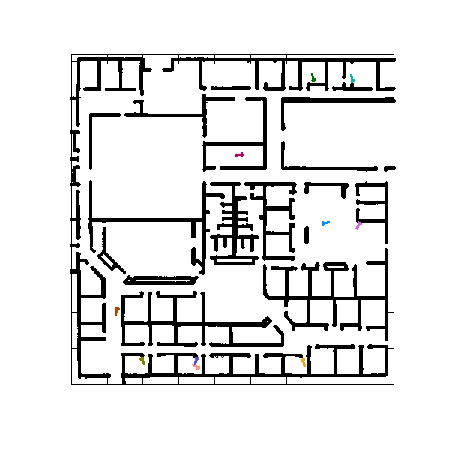
\includegraphics{./figures/parts/02/chapters/03/sections/04/map_willowgarage}}%
    \gplfronttext
  \end{picture}%
\endgroup

    %\caption{\small Ο χάρτης $\bm{M}_W$ του περιβάλλοντος WILLOWGARAGE}
    \label{fig:02_03_04:map_willowgarage}
  \end{subfigure}\\
  \begin{subfigure}{0.5\linewidth}
    \vspace{0.5cm}
    % GNUPLOT: LaTeX picture with Postscript
\begingroup
  \makeatletter
  \providecommand\color[2][]{%
    \GenericError{(gnuplot) \space\space\space\@spaces}{%
      Package color not loaded in conjunction with
      terminal option `colourtext'%
    }{See the gnuplot documentation for explanation.%
    }{Either use 'blacktext' in gnuplot or load the package
      color.sty in LaTeX.}%
    \renewcommand\color[2][]{}%
  }%
  \providecommand\includegraphics[2][]{%
    \GenericError{(gnuplot) \space\space\space\@spaces}{%
      Package graphicx or graphics not loaded%
    }{See the gnuplot documentation for explanation.%
    }{The gnuplot epslatex terminal needs graphicx.sty or graphics.sty.}%
    \renewcommand\includegraphics[2][]{}%
  }%
  \providecommand\rotatebox[2]{#2}%
  \@ifundefined{ifGPcolor}{%
    \newif\ifGPcolor
    \GPcolorfalse
  }{}%
  \@ifundefined{ifGPblacktext}{%
    \newif\ifGPblacktext
    \GPblacktexttrue
  }{}%
  % define a \g@addto@macro without @ in the name:
  \let\gplgaddtomacro\g@addto@macro
  % define empty templates for all commands taking text:
  \gdef\gplfronttext{}%
  \gdef\gplfronttext{}%
  \makeatother
  \ifGPblacktext
    % no textcolor at all
    \def\colorrgb#1{}%
    \def\colorgray#1{}%
  \else
    % gray or color?
    \ifGPcolor
      \def\colorrgb#1{\color[rgb]{#1}}%
      \def\colorgray#1{\color[gray]{#1}}%
      \expandafter\def\csname LTw\endcsname{\color{white}}%
      \expandafter\def\csname LTb\endcsname{\color{black}}%
      \expandafter\def\csname LTa\endcsname{\color{black}}%
      \expandafter\def\csname LT0\endcsname{\color[rgb]{1,0,0}}%
      \expandafter\def\csname LT1\endcsname{\color[rgb]{0,1,0}}%
      \expandafter\def\csname LT2\endcsname{\color[rgb]{0,0,1}}%
      \expandafter\def\csname LT3\endcsname{\color[rgb]{1,0,1}}%
      \expandafter\def\csname LT4\endcsname{\color[rgb]{0,1,1}}%
      \expandafter\def\csname LT5\endcsname{\color[rgb]{1,1,0}}%
      \expandafter\def\csname LT6\endcsname{\color[rgb]{0,0,0}}%
      \expandafter\def\csname LT7\endcsname{\color[rgb]{1,0.3,0}}%
      \expandafter\def\csname LT8\endcsname{\color[rgb]{0.5,0.5,0.5}}%
    \else
      % gray
      \def\colorrgb#1{\color{black}}%
      \def\colorgray#1{\color[gray]{#1}}%
      \expandafter\def\csname LTw\endcsname{\color{white}}%
      \expandafter\def\csname LTb\endcsname{\color{black}}%
      \expandafter\def\csname LTa\endcsname{\color{black}}%
      \expandafter\def\csname LT0\endcsname{\color{black}}%
      \expandafter\def\csname LT1\endcsname{\color{black}}%
      \expandafter\def\csname LT2\endcsname{\color{black}}%
      \expandafter\def\csname LT3\endcsname{\color{black}}%
      \expandafter\def\csname LT4\endcsname{\color{black}}%
      \expandafter\def\csname LT5\endcsname{\color{black}}%
      \expandafter\def\csname LT6\endcsname{\color{black}}%
      \expandafter\def\csname LT7\endcsname{\color{black}}%
      \expandafter\def\csname LT8\endcsname{\color{black}}%
    \fi
  \fi
  \setlength{\unitlength}{0.0500bp}%
  \begin{picture}(4000.00,4000.00)%
    \gplgaddtomacro\gplfronttext{%
      \colorrgb{0.00,0.00,0.00}%
      \put(388,1106){\makebox(0,0)[r]{\strut{}8}}%
      \colorrgb{0.00,0.00,0.00}%
      \put(388,1463){\makebox(0,0)[r]{\strut{}10}}%
      \colorrgb{0.00,0.00,0.00}%
      \put(388,1820){\makebox(0,0)[r]{\strut{}12}}%
      \colorrgb{0.00,0.00,0.00}%
      \put(388,2177){\makebox(0,0)[r]{\strut{}14}}%
      \colorrgb{0.00,0.00,0.00}%
      \put(388,2533){\makebox(0,0)[r]{\strut{}16}}%
      \colorrgb{0.00,0.00,0.00}%
      \put(388,2890){\makebox(0,0)[r]{\strut{}18}}%
      \colorrgb{0.00,0.00,0.00}%
      \put(388,3247){\makebox(0,0)[r]{\strut{}20}}%
      \colorrgb{0.00,0.00,0.00}%
      \put(527,610){\makebox(0,0){\strut{}4}}%
      \colorrgb{0.00,0.00,0.00}%
      \put(883,610){\makebox(0,0){\strut{}6}}%
      \colorrgb{0.00,0.00,0.00}%
      \put(1240,610){\makebox(0,0){\strut{}8}}%
      \colorrgb{0.00,0.00,0.00}%
      \put(1597,610){\makebox(0,0){\strut{}10}}%
      \colorrgb{0.00,0.00,0.00}%
      \put(1954,610){\makebox(0,0){\strut{}12}}%
      \colorrgb{0.00,0.00,0.00}%
      \put(2310,610){\makebox(0,0){\strut{}14}}%
      \colorrgb{0.00,0.00,0.00}%
      \put(2667,610){\makebox(0,0){\strut{}16}}%
      \colorrgb{0.00,0.00,0.00}%
      \put(3024,610){\makebox(0,0){\strut{}18}}%
      \colorrgb{0.00,0.00,0.00}%
      \put(3380,610){\makebox(0,0){\strut{}20}}%
      \colorrgb{0.00,0.00,0.00}%
      \put(-118,2069){\rotatebox{90}{\makebox(0,0){\strut{}$y$ [m]}}}%
      \colorrgb{0.00,0.00,0.00}%
      \put(2069,280){\makebox(0,0){\strut{}$x$ [m]}}%
      \put(2000,3600){\makebox(0,0){(ε') CSAL}}%
    }%
    \gplgaddtomacro\gplfronttext{%
    }%
    \put(0,0){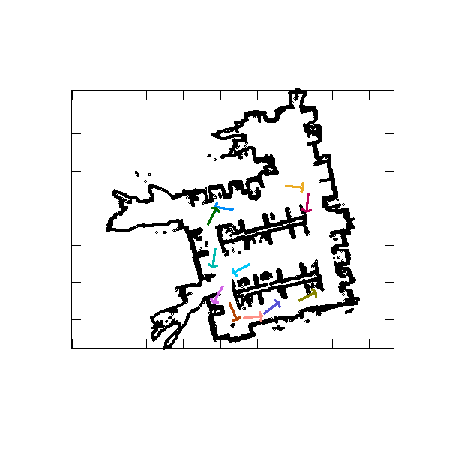
\includegraphics{./figures/parts/02/chapters/03/sections/04/map_csal}}%
    \gplfronttext
  \end{picture}%
\endgroup

    %\caption{\small Ο χάρτης $\bm{M}_A$ του περιβάλλοντος CSAL}
    \label{fig:02_03_04:map_csal}
  \end{subfigure}%
  \begin{subfigure}{0.5\linewidth}
    % GNUPLOT: LaTeX picture with Postscript
\begingroup
  \makeatletter
  \providecommand\color[2][]{%
    \GenericError{(gnuplot) \space\space\space\@spaces}{%
      Package color not loaded in conjunction with
      terminal option `colourtext'%
    }{See the gnuplot documentation for explanation.%
    }{Either use 'blacktext' in gnuplot or load the package
      color.sty in LaTeX.}%
    \renewcommand\color[2][]{}%
  }%
  \providecommand\includegraphics[2][]{%
    \GenericError{(gnuplot) \space\space\space\@spaces}{%
      Package graphicx or graphics not loaded%
    }{See the gnuplot documentation for explanation.%
    }{The gnuplot epslatex terminal needs graphicx.sty or graphics.sty.}%
    \renewcommand\includegraphics[2][]{}%
  }%
  \providecommand\rotatebox[2]{#2}%
  \@ifundefined{ifGPcolor}{%
    \newif\ifGPcolor
    \GPcolorfalse
  }{}%
  \@ifundefined{ifGPblacktext}{%
    \newif\ifGPblacktext
    \GPblacktexttrue
  }{}%
  % define a \g@addto@macro without @ in the name:
  \let\gplgaddtomacro\g@addto@macro
  % define empty templates for all commands taking text:
  \gdef\gplfronttext{}%
  \gdef\gplfronttext{}%
  \makeatother
  \ifGPblacktext
    % no textcolor at all
    \def\colorrgb#1{}%
    \def\colorgray#1{}%
  \else
    % gray or color?
    \ifGPcolor
      \def\colorrgb#1{\color[rgb]{#1}}%
      \def\colorgray#1{\color[gray]{#1}}%
      \expandafter\def\csname LTw\endcsname{\color{white}}%
      \expandafter\def\csname LTb\endcsname{\color{black}}%
      \expandafter\def\csname LTa\endcsname{\color{black}}%
      \expandafter\def\csname LT0\endcsname{\color[rgb]{1,0,0}}%
      \expandafter\def\csname LT1\endcsname{\color[rgb]{0,1,0}}%
      \expandafter\def\csname LT2\endcsname{\color[rgb]{0,0,1}}%
      \expandafter\def\csname LT3\endcsname{\color[rgb]{1,0,1}}%
      \expandafter\def\csname LT4\endcsname{\color[rgb]{0,1,1}}%
      \expandafter\def\csname LT5\endcsname{\color[rgb]{1,1,0}}%
      \expandafter\def\csname LT6\endcsname{\color[rgb]{0,0,0}}%
      \expandafter\def\csname LT7\endcsname{\color[rgb]{1,0.3,0}}%
      \expandafter\def\csname LT8\endcsname{\color[rgb]{0.5,0.5,0.5}}%
    \else
      % gray
      \def\colorrgb#1{\color{black}}%
      \def\colorgray#1{\color[gray]{#1}}%
      \expandafter\def\csname LTw\endcsname{\color{white}}%
      \expandafter\def\csname LTb\endcsname{\color{black}}%
      \expandafter\def\csname LTa\endcsname{\color{black}}%
      \expandafter\def\csname LT0\endcsname{\color{black}}%
      \expandafter\def\csname LT1\endcsname{\color{black}}%
      \expandafter\def\csname LT2\endcsname{\color{black}}%
      \expandafter\def\csname LT3\endcsname{\color{black}}%
      \expandafter\def\csname LT4\endcsname{\color{black}}%
      \expandafter\def\csname LT5\endcsname{\color{black}}%
      \expandafter\def\csname LT6\endcsname{\color{black}}%
      \expandafter\def\csname LT7\endcsname{\color{black}}%
      \expandafter\def\csname LT8\endcsname{\color{black}}%
    \fi
  \fi
  \setlength{\unitlength}{0.0500bp}%
  \begin{picture}(4000.00,4000.00)%
    \gplgaddtomacro\gplfronttext{%
      \colorrgb{0.00,0.00,0.00}%
      \put(1177,549){\makebox(0,0)[r]{\strut{}0}}%
      \colorrgb{0.00,0.00,0.00}%
      \put(1177,1092){\makebox(0,0)[r]{\strut{}5}}%
      \colorrgb{0.00,0.00,0.00}%
      \put(1177,1635){\makebox(0,0)[r]{\strut{}10}}%
      \colorrgb{0.00,0.00,0.00}%
      \put(1177,2178){\makebox(0,0)[r]{\strut{}15}}%
      \colorrgb{0.00,0.00,0.00}%
      \put(1177,2721){\makebox(0,0)[r]{\strut{}20}}%
      \colorrgb{0.00,0.00,0.00}%
      \put(1177,3264){\makebox(0,0)[r]{\strut{}25}}%
      \colorrgb{0.00,0.00,0.00}%
      \put(1418,220){\makebox(0,0){\strut{}0}}%
      \colorrgb{0.00,0.00,0.00}%
      \put(1635,220){\makebox(0,0){\strut{}2}}%
      \colorrgb{0.00,0.00,0.00}%
      \put(1852,220){\makebox(0,0){\strut{}4}}%
      \colorrgb{0.00,0.00,0.00}%
      \put(2069,220){\makebox(0,0){\strut{}6}}%
      \colorrgb{0.00,0.00,0.00}%
      \put(2286,220){\makebox(0,0){\strut{}8}}%
      \colorrgb{0.00,0.00,0.00}%
      \put(2503,220){\makebox(0,0){\strut{}10}}%
      \colorrgb{0.00,0.00,0.00}%
      \put(2790,220){\makebox(0,0){\strut{}12}}%
      \colorrgb{0.00,0.00,0.00}%
      \put(671,2069){\rotatebox{90}{\makebox(0,0){\strut{}$y$ [m]}}}%
      \colorrgb{0.00,0.00,0.00}%
      \put(2069,-110){\makebox(0,0){\strut{}$x$ [m]}}%
      \put(2100,3900){\makebox(0,0){(στ') LANDFILL}}%
    }%
    \gplgaddtomacro\gplfronttext{%
    }%
    \put(0,0){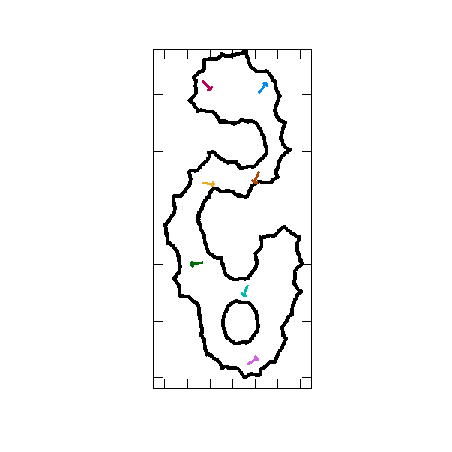
\includegraphics{./figures/parts/02/chapters/03/sections/04/map_dirtrack}}%
    \gplfronttext
  \end{picture}%
\endgroup

    %\caption{\small Ο χάρτης $\bm{M}_L$ του περιβάλλοντος LANDFILL}
    \label{fig:02_03_04:map_landfill}
  \end{subfigure}
\caption{\small Οι χάρτες των περιβαλλόντων στα οποία διενεργήθηκε η
         πειραματική διαδικασία}
\label{}
\end{figure}

Οι θέσεις στις οποίες τοποθετήθηκε το ρομπότ σε κάθε περιβάλλον καθορίστηκαν
από το σκοπό της αξιολόγησης του στόχου, δηλαδή στο περιβάλλον CORRIDOR το ρομπότ ήταν
τοποθετήθηκε κοντά στο ένα άκρο του, ώστε να αξιολογηθεί η απόκριση των μεθόδων σε
συμμετρία του περιβάλλοντος, κοντά στη μέση, ώστε να αξιολογηθεί η απόκρισή τους
σε σχέση με την ασάφεια του προσανατολισμού, και κοντά σε μια στροφή ώστε να αξιολογηθεί η
επίδραση της ανομοιομορφίας του περιβάλλοντος. Στο περιβάλλον HOME το ρομπότ ήταν
τοποθετήθηκε τυχαία και σε προκλητικές θέσεις, κοντά ή μακριά από το
αντικείμενα, και σε θέσεις των οποίων το περιβάλλον ήταν σχεδόν παρόμοιο με άλλα μέρη του
του περιβάλλοντος. Στο περιβάλλον WAREHOUSE τοποθετήθηκε με τρόπους που ένα
θα περίμενε κανείς ότι η λειτουργία του ρομπότ θα ξεκινούσε για πρώτη φορά, και στο
θέσεις τέτοιες που θα προκαλούσαν την απόκριση των μεθόδων σε ελλείψεις εύρους
ακτίνων (ένας τυπικός αισθητήρας LIDAR αναφέρει μια ένδειξη μέγιστης εμβέλειας όταν η εν λόγω ακτίνα
δεν συναντά αντικείμενα στην πορεία της). Στο περιβάλλον WILLOWGARAGE το ρομπότ
τοποθετήθηκε σε δωμάτια που ήταν είτε πανομοιότυπα είτε σχεδόν πανομοιότυπα με άλλα
και τυχαία. Ο προσανατολισμός της πραγματικής θέσης του ρομπότ δεν έχει καμία σημασία
δεδομένου ότι ο αισθητήρας εύρεσης απόστασης είναι πανοραμικός, και καθορίστηκε τυχαία από το
δειγματοληψία από μια ομοιόμορφη κατανομή $U(-\pi,\pi)$. Πίνακας
\ref{tbl:true_poses_simulation} δείχνει την τοποθέτηση των θέσεων σε κάθε
προσομοιωμένο περιβάλλον/χάρτη, μαζί με τους δείκτες τους στα επόμενα σχήματα.
Ο πίνακας \ref{tbl:true_poses_experiment} δείχνει την τοποθέτηση των θέσεων στο
περιβάλλον/χάρτη του CSAL. Λόγω της έλλειψης υποδομής που θα μπορούσε να μετρήσει
τη στάση του ρομπότ στο πραγματικό περιβάλλον CSAL (π.χ. ένα σύστημα MoCap), η
πόζα του ρομπότ εκτιμήθηκε με τη χρήση ενός φίλτρου σωματιδίων (MCL) και
ως εκ τούτου μπορεί να υπόκειται σε αναπόφευκτα σφάλματα εκτίμησης της ίδιας της πόζας.

\begin{table}\centering
  \begin{tabular} {c|llll} \midrule
    pose id & $x$ [m]   & $y$  [m]  & $\theta$ [rad]  &  sign            \\ \midrule
    \multicolumn{5}{c}{CORRIDOR}                                         \\ \midrule
    $\bm{p}_a^C$   & $11.56$   & $12.2$    & $-0.79$         & $+$       \\
    $\bm{p}_b^C$   & $12.06$   & $8.2$     & $2.01$          & $\circ$   \\
    $\bm{p}_c^C$   & $8.06$    & $9.20$    & $-3.28$         & $\ast$    \\ \midrule
    \multicolumn{5}{c}{HOME}                                             \\ \midrule
    $\bm{p}_a^H$   & $14.44$   & $24.04$   & $0.065$         & $+$       \\
    $\bm{p}_b^H$   & $17.84$   & $24.84$   & $1.33$          & $\circ$   \\
    $\bm{p}_c^H$   & $15.0$    & $14.68$   & $0.68$          & $\ast$    \\
    $\bm{p}_d^H$   & $22.0$    & $14.22$   & $-2.66$         & $\cdot$   \\
    $\bm{p}_e^H$   & $26.0$    & $16.10$   & $0.69$          & $\times$  \\
    $\bm{p}_f^H$   & $24.46$   & $9.68$    & $-0.49$         & $\square$ \\
    $\bm{p}_g^H$   & $18.26$   & $11.02$   & $-3.10$         & $\diamond$\\
    $\bm{p}_h^H$   & $27.64$   & $7.78$    & $-0.14$         & $\wedge$  \\
    $\bm{p}_i^H$   & $24.28$   & $21.44$   & $2.41$          & $\vee$    \\
    $\bm{p}_j^H$   & $29.0$    & $28.64$   & $0.31$          & $>$       \\
    $\bm{p}_k^H$   & $31.0$    & $12.2$    & $-2.19$         & $<$       \\ \midrule
    \multicolumn{5}{c}{WAREHOUSE}                                        \\ \midrule
    $\bm{p}_a^W$   & $8.08$    & $3.02$    & $-2.85$         & $+$       \\
    $\bm{p}_b^W$   & $35.16$   & $15.25$   & $-2.20$         & $\circ$   \\
    $\bm{p}_c^W$   & $38.81$   & $2.35$    & $1.36$          & $\ast$    \\
    $\bm{p}_d^W$   & $33.42$   & $4.92$    & $2.78$          & $\cdot$   \\
    $\bm{p}_e^W$   & $17.08$   & $8.75$    & $2.83$          & $\times$  \\
    $\bm{p}_f^W$   & $8.63$    & $11.93$   & $-1.26$         & $\square$ \\
    $\bm{p}_g^W$   & $1.27$    & $9.5$     & $0.239$         & $\diamond$\\ \midrule
    \multicolumn{5}{c}{WILLOWGARAGE}                                     \\ \midrule
    $\bm{p}_a^G$   & $77.56$   & $37.48$   & $-1.27$         & $+$       \\
    $\bm{p}_b^G$   & $67.85$   & $66.90$   & $0.13$          & $\circ$   \\
    $\bm{p}_c^G$   & $81.0$    & $57.60$   & $-2.97$         & $\ast$    \\
    $\bm{p}_d^G$   & $78.55$   & $78.35$   & $-1.31$         & $\cdot$   \\
    $\bm{p}_e^G$   & $84.0$    & $78.15$   & $0.94$          & $\times$  \\
    $\bm{p}_f^G$   & $84.75$   & $56.65$   & $1.02$          & $\square$ \\
    $\bm{p}_g^G$   & $51.15$   & $44.65$   & $1.29$          & $\diamond$\\
    $\bm{p}_h^G$   & $61.95$   & $37.80$   & $-0.58$         & $\wedge$  \\
    $\bm{p}_i^G$   & $62.20$   & $37.76$   & $-1.22$         & $\vee$    \\
    $\bm{p}_j^G$   & $55.20$   & $37.76$   & $0.91$          & $>$       \\ \midrule
    \multicolumn{5}{c}{LANDFILL}                                         \\ \midrule
    $\bm{p}_a^L$   & $3.34$    & $17.19$   & $-0.082$        & $+$       \\
    $\bm{p}_b^L$   & $3.34$    & $26.19$   & $-0.78$         & $\circ$   \\
    $\bm{p}_c^L$   & $8.34$    & $25.19$   & $0.90$          & $\ast$    \\
    $\bm{p}_d^L$   & $3.34$    & $10.19$   & $-2.97$         & $\cdot$   \\
    $\bm{p}_e^L$   & $7.34$    & $8.19$    & $-1.93$         & $\times$  \\
    $\bm{p}_f^L$   & $7.34$    & $1.19$    & $0.58$          & $\square$ \\
    $\bm{p}_g^L$   & $8.34$    & $18.19$   & $-2.02$         & $\diamond$\\ \bottomrule
  \end{tabular}
  \caption{\small The robot's true poses tested per simulated environment and
           the sign by which they are referred to in figures}
  \label{tbl:true_poses_simulation}
\end{table}

\begin{table}\centering
  \begin{tabular} {c|lll} \midrule
    pose id & $x$ [m]   & $y$  [m]  & $\theta$ [rad]         \\ \midrule
    \multicolumn{4}{c}{CSAL AUTh}                            \\ \midrule
    $\bm{p}_a^A$   & $15.47$   & $15.19$   & $-0.09$         \\
    $\bm{p}_b^A$   & $16.72$   & $14.81$   & $-1.67$         \\
    $\bm{p}_c^A$   & $12.67$   & $13.91$   & $2.98$          \\
    $\bm{p}_d^A$   & $11.30$   & $13.10$   & $1.08$          \\
    $\bm{p}_e^A$   & $11.71$   & $11.83$   & $-1.70$         \\
    $\bm{p}_f^A$   & $12.12$   & $9.80$    & $-2.08$         \\
    $\bm{p}_g^A$   & $12.47$   & $8.89$    & $-1.14$         \\
    $\bm{p}_h^A$   & $13.22$   & $8.08$    & $0.10$          \\
    $\bm{p}_i^A$   & $14.32$   & $8.31$    & $0.65$          \\
    $\bm{p}_j^A$   & $16.22$   & $9.01$    & $0.47$          \\
    $\bm{p}_k^A$   & $13.56$   & $10.99$   & $-2.63$         \\ \midrule
  \end{tabular}
  \caption{\small The robot's true poses tested in the real environment of CSAL
           AUTh and their corresponding identifiers}
  \label{tbl:true_poses_experiment}
\end{table}


Δεδομένης της παρατήρησης \ref{rem:accuracy}, μια σωστή συνολική λύση πόζας θεωρήθηκε ως
όταν η απόκλιση της θέσης της από τη θέση της πραγματικής πόζας ήταν
μικρότερη από $1.0$ m.\footnote{Η τιμή της αυθαίρετης ακραίας/αποκλίσεως
ορίστηκε ως τέτοιο μετά από πειράματα σε πραγματικές συνθήκες
με το ίδιο ρομπότ, όταν χρησιμοποιήθηκε ο εντοπισμός Monte Carlo (MCL) για την πόζα
για την παρακολούθηση της στάσης. Η μεθοδολογία ήταν η εξής: πρώτα ο παρεχόμενος αρχικός
εκτίμηση της θέσης του ρομπότ ρυθμίστηκε σε μια δεδομένη μετατόπιση από την πραγματική του θέση.
θέση. Στη συνέχεια, το ρομπότ ανέλαβε να πλοηγηθεί αυτόνομα σε ένα σύνολο
θέση στο χάρτη χρησιμοποιώντας την εκτίμηση της θέσης του MCL ως θέση του ρομπότ. Εάν το ρομπότ
δεν κατάφερνε να φτάσει στην καθορισμένη θέση, η μετατόπιση μειωνόταν έως ότου
το έκανε επανειλημμένα}

Όσοι διέμεναν εκτός αυτού του κύκλου ονομάζονται στο εξής ακραίοι.  Κανένα σφάλμα
κατώφλι τοποθετήθηκε στον προσανατολισμό, καθώς δεν είναι βέβαιο ότι ένα πιθανοτικό
μέθοδος εντοπισμού της στάσης, που χρησιμοποιείται στη συνέχεια του παγκόσμιου εντοπισμού, δεν θα μπορούσε να
περαιτέρω εντοπισμό του ρομπότ και την παρακολούθηση της στάσης του.  Όσον αφορά το μέγεθος του
του συνόλου υποθέσεων $\mathcal{H}$ των υποθέσεων που είναι διασκορπισμένες σε κάθε
περιβάλλον, ανάλογα με την παρατήρηση \ref{rem:hypotheses_number}, καμία μέθοδος δεν ήταν
δεν υπήρξε καμία μέθοδος που να στερείται ταυτοτήτων σε κανένα περιβάλλον: για τα περιβάλλοντα CORRIDOR, LANDFILL,
και CSAL $|\mathcal{H}_C| = |\mathcal{H}_L| = |\mathcal{H}_A| = 100$- για τα περιβάλλοντα
περιβάλλοντα HOME και WAREHOUSE $|\mathcal{H}_H| = |\mathcal{H}_W| = 200$- για
περιβάλλον WILLOWGARAGE $|\mathcal{H}_G| = 500$.  Τα κατώτατα όρια κλίμακας ήταν
τέθηκαν σε $(\underline{\sigma}, \overline{\sigma}) = (0.9, 1.2)$. Το πλάτος και το
ύψος των εικόνων που εισάγονται στο FMI-SPOMF ορίστηκε σε $N_G = 2^8$.
δοκιμές έδειξαν ότι αυτή η ρύθμιση είχε ως αποτέλεσμα τόσο χαμηλούς χρόνους εκτέλεσης όσο και
ακριβή διάκριση μεταξύ αληθών και ψευδώς θετικών λύσεων. Υψηλότερες τιμές
του $N_G$ θα αύξαναν την ευαισθησία της μεθόδου όσον αφορά τη διάκριση
μεταξύ θέσεων που έχουν οριστεί σε παρόμοιο περιβάλλον, αλλά με κόστος την αύξηση της εκτέλεσης
χρόνο εκτέλεσης.

Όλες οι προσομοιώσεις πραγματοποιήθηκαν στο Gazebo
environment\footnote{\url{https://www.gazebosim.org/}} μέσω
ROS\footnote{\url{https://www.ros.org/}}, σε C++ και Ubuntu 16.04, με ένα
επεξεργαστή με 12 νήματα, που λειτουργεί στα 4,00 GHz, χρησιμοποιώντας έως και $32$Gb μνήμης RAM. Χάρτες της
προσομοιωμένων περιβαλλόντων κατασκευάστηκαν χρησιμοποιώντας το \texttt{slam\_karto} του ROS.
package\footnote{\url{http://wiki.ros.org/slam\_karto}}. Όλα τα πειράματα ήταν
πραγματοποιήθηκαν με έναν επεξεργαστή 8 νημάτων, που εκτελούσε στα 2,30 GHz, χρησιμοποιώντας έως και
$8$Gb μνήμης RAM. Ο χάρτης του περιβάλλοντος CSAL κατασκευάστηκε με τη χρήση του προγράμματος ROS
\texttt{gmapping} πακέτο\footnote{\url{http://wiki.ros.org/gmapping}}. Ως
σημείωση εφαρμογής όσον αφορά τους χάρτες και τη χαρτογράφηση, τονίζουμε την προσοχή στο ότι
το αποτέλεσμα του αλγορίθμου χαρτογράφησης μπορεί να είναι ατελές με την έννοια ότι οι ελεύθερες
χώρος μπορεί να εισαχθεί μεταξύ της συνέχειας ακόμη και ενός μεμονωμένου
εμποδίου.\footnote{ Ατέλειες αυτού του τύπου οφείλονται στη διακριτή φύση
του αισθητήρα εμβέλειας όσον αφορά τη γωνιακή δειγματοληψία, τους ζητούμενους χάρτες
ανάλυση, ή στο χρόνο εκτέλεσης του αλγορίθμου σε σύγκριση με τον όγκο της εισόδου.
πληροφορίες} Αυτό το είδος δομικού σφάλματος μπορεί να αλλοιώσει το αποτέλεσμα του
σάρωσης-προς-χάρτη-σάρωσης, και ως εκ τούτου πρέπει να δίνεται προσοχή ώστε είτε
οι χάρτες να είναι σωστοί από προεπιλογή, ή να διορθώνεται ο λανθασμένα δημιουργημένος ελεύθερος χώρος
\footnote{ Σκεφτείτε για παράδειγμα την περίπτωση όπου ένας τοίχος χωρίζει έναν
δωμάτιο από ένα άλλο. Στην περίπτωση ενός χάρτη πλέγματος πληρότητας η εισαγωγή του
ελεύθερου χώρου ως "ρωγμή" στον τοίχο θα οδηγούσε σε μια κατάσταση όπου, εάν ένα
εικονική σάρωση γίνεται σε απόσταση από τον τοίχο που βρίσκεται εντός του εύρους
αισθητήρα, τουλάχιστον μία ακτίνα μπορεί να διαρρεύσει μέσα από τη ρωγμή και να αναφέρει
λανθασμένη μέτρηση της εμβέλειας.  Η συμπεριφορά αυτή μπορεί να επιδεινωθεί εάν ο τοίχος αυτός
διαχωρίζει τη χαρτογραφημένη περιοχή με τη μη χαρτογραφημένη περιοχή και ο
ρουτίνα εύρεσης τομής δεν έχει σχεδιαστεί για να χειρίζεται μη σημασμένο χώρο} Για την
εφαρμογή του 2D μετασχηματισμού Fourier-Mellin η \texttt{imgreg\_dft}
python modules were used.\footnote{\url{https://pypi.org/project/imreg\_dft/}}
Όσον αφορά τις εισόδους του, αυτές ήταν εικόνες που παρήχθησαν μέσω του \texttt{GNU Octave}
v.4.0.0:\footnote{https://www.gnu.org/software/octave/} πραγματικές και εικονικές σαρώσεις
απεικονίστηκαν σε τυπικό μέγεθος εικονοστοιχείου $N_G \times N_G$ και στη συνέχεια γράφτηκαν στο δίσκο
ως εικόνες \texttt{.png}. Εικόνες των μορφών \texttt{.gif}, \texttt{.jpg}, και
\texttt{.tiff} δεν παρήγαγαν επαρκή αποτελέσματα. Μια καθυστέρηση μεταξύ της παραγωγής μιας
εικόνας και της επεξεργασίας μιας υπόθεσης πόζας ήταν απαραίτητη προκειμένου οι εικόνες να είναι
Οι χρόνοι εκτέλεσης της PGL-FMIC στο υποτμήμα
\ref{subsec:exec_times} αντικατοπτρίζει τους καθαρούς χρόνους εκτέλεσης του αλγορίθμου ανά
υπόθεση. Το υπολογιστικό κόστος της προτεινόμενης μεθόδου ήταν 483MB (συμπεριλαμβανομένων των
\texttt{Octave}) στη μνήμη και περίπου $25\%$ χρήση ενός πυρήνα CPU.


Στις επόμενες ενότητες παρουσιάζονται τα αποτελέσματα των προσομοιώσεων που πραγματοποιήθηκαν με
την προτεινόμενη μέθοδο (PGL-FMIC) και έναν αλγόριθμο τελευταίας τεχνολογίας (PLICP) για
την επίλυση του ίδιου προβλήματος του παγκόσμιου εντοπισμού υπό συνθήκες ακινησίας στο
παραπάνω έξι περιβάλλοντα υπό τις συνθήκες που περιγράφονται.






%%%%%%%%%%%%%%%%%%%%%%%%%%%%%%%%%%%%%%%%%%%%%%%%%%%%%%%%%%%%%%%%%%%%%%%%%%%%%%%%
\subsection{Αποτελέσματα}
\label{subsection:02_03_04:02}

\begin{figure}
  \hspace{-1.5cm}
  % GNUPLOT: LaTeX picture with Postscript
\begingroup
  \makeatletter
  \providecommand\color[2][]{%
    \GenericError{(gnuplot) \space\space\space\@spaces}{%
      Package color not loaded in conjunction with
      terminal option `colourtext'%
    }{See the gnuplot documentation for explanation.%
    }{Either use 'blacktext' in gnuplot or load the package
      color.sty in LaTeX.}%
    \renewcommand\color[2][]{}%
  }%
  \providecommand\includegraphics[2][]{%
    \GenericError{(gnuplot) \space\space\space\@spaces}{%
      Package graphicx or graphics not loaded%
    }{See the gnuplot documentation for explanation.%
    }{The gnuplot epslatex terminal needs graphicx.sty or graphics.sty.}%
    \renewcommand\includegraphics[2][]{}%
  }%
  \providecommand\rotatebox[2]{#2}%
  \@ifundefined{ifGPcolor}{%
    \newif\ifGPcolor
    \GPcolorfalse
  }{}%
  \@ifundefined{ifGPblacktext}{%
    \newif\ifGPblacktext
    \GPblacktexttrue
  }{}%
  % define a \g@addto@macro without @ in the name:
  \let\gplgaddtomacro\g@addto@macro
  % define empty templates for all commands taking text:
  \gdef\gplfronttext{}%
  \gdef\gplfronttext{}%
  \makeatother
  \ifGPblacktext
    % no textcolor at all
    \def\colorrgb#1{}%
    \def\colorgray#1{}%
  \else
    % gray or color?
    \ifGPcolor
      \def\colorrgb#1{\color[rgb]{#1}}%
      \def\colorgray#1{\color[gray]{#1}}%
      \expandafter\def\csname LTw\endcsname{\color{white}}%
      \expandafter\def\csname LTb\endcsname{\color{black}}%
      \expandafter\def\csname LTa\endcsname{\color{black}}%
      \expandafter\def\csname LT0\endcsname{\color[rgb]{1,0,0}}%
      \expandafter\def\csname LT1\endcsname{\color[rgb]{0,1,0}}%
      \expandafter\def\csname LT2\endcsname{\color[rgb]{0,0,1}}%
      \expandafter\def\csname LT3\endcsname{\color[rgb]{1,0,1}}%
      \expandafter\def\csname LT4\endcsname{\color[rgb]{0,1,1}}%
      \expandafter\def\csname LT5\endcsname{\color[rgb]{1,1,0}}%
      \expandafter\def\csname LT6\endcsname{\color[rgb]{0,0,0}}%
      \expandafter\def\csname LT7\endcsname{\color[rgb]{1,0.3,0}}%
      \expandafter\def\csname LT8\endcsname{\color[rgb]{0.5,0.5,0.5}}%
    \else
      % gray
      \def\colorrgb#1{\color{black}}%
      \def\colorgray#1{\color[gray]{#1}}%
      \expandafter\def\csname LTw\endcsname{\color{white}}%
      \expandafter\def\csname LTb\endcsname{\color{black}}%
      \expandafter\def\csname LTa\endcsname{\color{black}}%
      \expandafter\def\csname LT0\endcsname{\color{black}}%
      \expandafter\def\csname LT1\endcsname{\color{black}}%
      \expandafter\def\csname LT2\endcsname{\color{black}}%
      \expandafter\def\csname LT3\endcsname{\color{black}}%
      \expandafter\def\csname LT4\endcsname{\color{black}}%
      \expandafter\def\csname LT5\endcsname{\color{black}}%
      \expandafter\def\csname LT6\endcsname{\color{black}}%
      \expandafter\def\csname LT7\endcsname{\color{black}}%
      \expandafter\def\csname LT8\endcsname{\color{black}}%
    \fi
  \fi
  \setlength{\unitlength}{0.0500bp}%
  \begin{picture}(11000.00,12000.00)%
    \gplgaddtomacro\gplfronttext{%
      \colorrgb{0.00,0.00,0.00}%
      \put(1431,10003){\makebox(0,0)[r]{\strut{}\small $0\%$}}%
      \colorrgb{0.00,0.00,0.00}%
      \put(1431,10277){\makebox(0,0)[r]{\strut{}\small $25\%$}}%
      \colorrgb{0.00,0.00,0.00}%
      \put(1431,10551){\makebox(0,0)[r]{\strut{}\small $50\%$}}%
      \colorrgb{0.00,0.00,0.00}%
      \put(1431,10825){\makebox(0,0)[r]{\strut{}\small $75\%$}}%
      \colorrgb{0.00,0.00,0.00}%
      \put(1431,11099){\makebox(0,0)[r]{\strut{}\small $100\%$}}%
      \colorrgb{0.00,0.00,0.00}%
      \put(2162,9783){\makebox(0,0){\strut{}\small $\bm{p}_a^C$}}%
      \colorrgb{0.00,0.00,0.00}%
      \put(3360,9783){\makebox(0,0){\strut{}\small $\bm{p}_b^C$}}%
      \colorrgb{0.00,0.00,0.00}%
      \put(4557,9783){\makebox(0,0){\strut{}\small $\bm{p}_c^C$}}%
      \colorrgb{0.00,0.00,0.00}%
      \put(465,10551){\rotatebox{90}{\makebox(0,0){\strut{}\small CORRIDOR}}}%
      \colorrgb{0.00,0.00,0.00}%
      \put(3359,11429){\makebox(0,0){\strut{}PLICP}}%
    }%
    \gplgaddtomacro\gplfronttext{%
    }%
    \gplgaddtomacro\gplfronttext{%
      \colorrgb{0.00,0.00,0.00}%
      \put(6096,10003){\makebox(0,0)[r]{\strut{}\small $0\%$}}%
      \colorrgb{0.00,0.00,0.00}%
      \put(6096,10277){\makebox(0,0)[r]{\strut{}\small $25\%$}}%
      \colorrgb{0.00,0.00,0.00}%
      \put(6096,10551){\makebox(0,0)[r]{\strut{}\small $50\%$}}%
      \colorrgb{0.00,0.00,0.00}%
      \put(6096,10825){\makebox(0,0)[r]{\strut{}\small $75\%$}}%
      \colorrgb{0.00,0.00,0.00}%
      \put(6096,11099){\makebox(0,0)[r]{\strut{}\small $100\%$}}%
      \colorrgb{0.00,0.00,0.00}%
      \put(6827,9783){\makebox(0,0){\strut{}\small $\bm{p}_a^C$}}%
      \colorrgb{0.00,0.00,0.00}%
      \put(8024,9783){\makebox(0,0){\strut{}\small $\bm{p}_b^C$}}%
      \colorrgb{0.00,0.00,0.00}%
      \put(9221,9783){\makebox(0,0){\strut{}\small $\bm{p}_c^C$}}%
      \colorrgb{0.00,0.00,0.00}%
      \put(8024,11429){\makebox(0,0){\strut{}PGL-FMIC}}%
    }%
    \gplgaddtomacro\gplfronttext{%
    }%
    \gplgaddtomacro\gplfronttext{%
      \colorrgb{0.00,0.00,0.00}%
      \put(1431,8266){\makebox(0,0)[r]{\strut{}\small $0\%$}}%
      \colorrgb{0.00,0.00,0.00}%
      \put(1431,8540){\makebox(0,0)[r]{\strut{}\small $25\%$}}%
      \colorrgb{0.00,0.00,0.00}%
      \put(1431,8814){\makebox(0,0)[r]{\strut{}\small $50\%$}}%
      \colorrgb{0.00,0.00,0.00}%
      \put(1431,9088){\makebox(0,0)[r]{\strut{}\small $75\%$}}%
      \colorrgb{0.00,0.00,0.00}%
      \put(1431,9362){\makebox(0,0)[r]{\strut{}\small $100\%$}}%
      \colorrgb{0.00,0.00,0.00}%
      \put(1726,8046){\makebox(0,0){\strut{}\small $\bm{p}_a^H$}}%
      \colorrgb{0.00,0.00,0.00}%
      \put(2053,8046){\makebox(0,0){\strut{}\small $\bm{p}_b^H$}}%
      \colorrgb{0.00,0.00,0.00}%
      \put(2380,8046){\makebox(0,0){\strut{}\small $\bm{p}_c^H$}}%
      \colorrgb{0.00,0.00,0.00}%
      \put(2706,8046){\makebox(0,0){\strut{}\small $\bm{p}_d^H$}}%
      \colorrgb{0.00,0.00,0.00}%
      \put(3033,8046){\makebox(0,0){\strut{}\small $\bm{p}_e^H$}}%
      \colorrgb{0.00,0.00,0.00}%
      \put(3360,8046){\makebox(0,0){\strut{}\small $\bm{p}_f^H$}}%
      \colorrgb{0.00,0.00,0.00}%
      \put(3686,8046){\makebox(0,0){\strut{}\small $\bm{p}_g^H$}}%
      \colorrgb{0.00,0.00,0.00}%
      \put(4013,8046){\makebox(0,0){\strut{}\small $\bm{p}_h^H$}}%
      \colorrgb{0.00,0.00,0.00}%
      \put(4339,8046){\makebox(0,0){\strut{}\small $\bm{p}_i^H$}}%
      \colorrgb{0.00,0.00,0.00}%
      \put(4666,8046){\makebox(0,0){\strut{}\small $\bm{p}_j^H$}}%
      \colorrgb{0.00,0.00,0.00}%
      \put(4993,8046){\makebox(0,0){\strut{}\small $\bm{p}_k^H$}}%
      \colorrgb{0.00,0.00,0.00}%
      \put(465,8814){\rotatebox{90}{\makebox(0,0){\strut{}\small HOME}}}%
    }%
    \gplgaddtomacro\gplfronttext{%
    }%
    \gplgaddtomacro\gplfronttext{%
      \colorrgb{0.00,0.00,0.00}%
      \put(6096,8266){\makebox(0,0)[r]{\strut{}\small $0\%$}}%
      \colorrgb{0.00,0.00,0.00}%
      \put(6096,8540){\makebox(0,0)[r]{\strut{}\small $25\%$}}%
      \colorrgb{0.00,0.00,0.00}%
      \put(6096,8814){\makebox(0,0)[r]{\strut{}\small $50\%$}}%
      \colorrgb{0.00,0.00,0.00}%
      \put(6096,9088){\makebox(0,0)[r]{\strut{}\small $75\%$}}%
      \colorrgb{0.00,0.00,0.00}%
      \put(6096,9362){\makebox(0,0)[r]{\strut{}\small $100\%$}}%
      \colorrgb{0.00,0.00,0.00}%
      \put(6391,8046){\makebox(0,0){\strut{}}}%
      \colorrgb{0.00,0.00,0.00}%
      \put(6718,8046){\makebox(0,0){\strut{}}}%
      \colorrgb{0.00,0.00,0.00}%
      \put(7044,8046){\makebox(0,0){\strut{}}}%
      \colorrgb{0.00,0.00,0.00}%
      \put(7371,8046){\makebox(0,0){\strut{}}}%
      \colorrgb{0.00,0.00,0.00}%
      \put(7697,8046){\makebox(0,0){\strut{}}}%
      \colorrgb{0.00,0.00,0.00}%
      \put(8024,8046){\makebox(0,0){\strut{}}}%
      \colorrgb{0.00,0.00,0.00}%
      \put(8351,8046){\makebox(0,0){\strut{}}}%
      \colorrgb{0.00,0.00,0.00}%
      \put(8677,8046){\makebox(0,0){\strut{}}}%
      \colorrgb{0.00,0.00,0.00}%
      \put(9004,8046){\makebox(0,0){\strut{}}}%
      \colorrgb{0.00,0.00,0.00}%
      \put(9330,8046){\makebox(0,0){\strut{}}}%
      \colorrgb{0.00,0.00,0.00}%
      \put(9657,8046){\makebox(0,0){\strut{}}}%
    }%
    \gplgaddtomacro\gplfronttext{%
    }%
    \gplgaddtomacro\gplfronttext{%
      \colorrgb{0.00,0.00,0.00}%
      \put(1431,6530){\makebox(0,0)[r]{\strut{}\small $0\%$}}%
      \colorrgb{0.00,0.00,0.00}%
      \put(1431,6804){\makebox(0,0)[r]{\strut{}\small $25\%$}}%
      \colorrgb{0.00,0.00,0.00}%
      \put(1431,7078){\makebox(0,0)[r]{\strut{}\small $50\%$}}%
      \colorrgb{0.00,0.00,0.00}%
      \put(1431,7352){\makebox(0,0)[r]{\strut{}\small $75\%$}}%
      \colorrgb{0.00,0.00,0.00}%
      \put(1431,7626){\makebox(0,0)[r]{\strut{}\small $100\%$}}%
      \colorrgb{0.00,0.00,0.00}%
      \put(1820,6310){\makebox(0,0){\strut{}\small $\bm{p}_a^W$}}%
      \colorrgb{0.00,0.00,0.00}%
      \put(2333,6310){\makebox(0,0){\strut{}\small $\bm{p}_b^W$}}%
      \colorrgb{0.00,0.00,0.00}%
      \put(2846,6310){\makebox(0,0){\strut{}\small $\bm{p}_c^W$}}%
      \colorrgb{0.00,0.00,0.00}%
      \put(3360,6310){\makebox(0,0){\strut{}\small $\bm{p}_d^W$}}%
      \colorrgb{0.00,0.00,0.00}%
      \put(3873,6310){\makebox(0,0){\strut{}\small $\bm{p}_e^W$}}%
      \colorrgb{0.00,0.00,0.00}%
      \put(4386,6310){\makebox(0,0){\strut{}\small $\bm{p}_f^W$}}%
      \colorrgb{0.00,0.00,0.00}%
      \put(4899,6310){\makebox(0,0){\strut{}\small $\bm{p}_g^W$}}%
      \colorrgb{0.00,0.00,0.00}%
      \put(465,7078){\rotatebox{90}{\makebox(0,0){\strut{}\small WAREHOUSE}}}%
    }%
    \gplgaddtomacro\gplfronttext{%
    }%
    \gplgaddtomacro\gplfronttext{%
      \colorrgb{0.00,0.00,0.00}%
      \put(6096,6530){\makebox(0,0)[r]{\strut{}\small $0\%$}}%
      \colorrgb{0.00,0.00,0.00}%
      \put(6096,6804){\makebox(0,0)[r]{\strut{}\small $25\%$}}%
      \colorrgb{0.00,0.00,0.00}%
      \put(6096,7078){\makebox(0,0)[r]{\strut{}\small $50\%$}}%
      \colorrgb{0.00,0.00,0.00}%
      \put(6096,7352){\makebox(0,0)[r]{\strut{}\small $75\%$}}%
      \colorrgb{0.00,0.00,0.00}%
      \put(6096,7626){\makebox(0,0)[r]{\strut{}\small $100\%$}}%
      \colorrgb{0.00,0.00,0.00}%
      \put(6485,6310){\makebox(0,0){\strut{}\small $\bm{p}_a^W$}}%
      \colorrgb{0.00,0.00,0.00}%
      \put(6998,6310){\makebox(0,0){\strut{}\small $\bm{p}_b^W$}}%
      \colorrgb{0.00,0.00,0.00}%
      \put(7511,6310){\makebox(0,0){\strut{}\small $\bm{p}_c^W$}}%
      \colorrgb{0.00,0.00,0.00}%
      \put(8024,6310){\makebox(0,0){\strut{}\small $\bm{p}_d^W$}}%
      \colorrgb{0.00,0.00,0.00}%
      \put(8537,6310){\makebox(0,0){\strut{}\small $\bm{p}_e^W$}}%
      \colorrgb{0.00,0.00,0.00}%
      \put(9050,6310){\makebox(0,0){\strut{}\small $\bm{p}_f^W$}}%
      \colorrgb{0.00,0.00,0.00}%
      \put(9563,6310){\makebox(0,0){\strut{}\small $\bm{p}_g^W$}}%
    }%
    \gplgaddtomacro\gplfronttext{%
    }%
    \gplgaddtomacro\gplfronttext{%
      \colorrgb{0.00,0.00,0.00}%
      \put(1431,4793){\makebox(0,0)[r]{\strut{}\small $0\%$}}%
      \colorrgb{0.00,0.00,0.00}%
      \put(1431,5067){\makebox(0,0)[r]{\strut{}\small $25\%$}}%
      \colorrgb{0.00,0.00,0.00}%
      \put(1431,5341){\makebox(0,0)[r]{\strut{}\small $50\%$}}%
      \colorrgb{0.00,0.00,0.00}%
      \put(1431,5615){\makebox(0,0)[r]{\strut{}\small $75\%$}}%
      \colorrgb{0.00,0.00,0.00}%
      \put(1431,5889){\makebox(0,0)[r]{\strut{}\small $100\%$}}%
      \colorrgb{0.00,0.00,0.00}%
      \put(1743,4573){\makebox(0,0){\strut{}\small $\bm{p}_a^G$}}%
      \colorrgb{0.00,0.00,0.00}%
      \put(2102,4573){\makebox(0,0){\strut{}\small $\bm{p}_b^G$}}%
      \colorrgb{0.00,0.00,0.00}%
      \put(2461,4573){\makebox(0,0){\strut{}\small $\bm{p}_c^G$}}%
      \colorrgb{0.00,0.00,0.00}%
      \put(2821,4573){\makebox(0,0){\strut{}\small $\bm{p}_d^G$}}%
      \colorrgb{0.00,0.00,0.00}%
      \put(3180,4573){\makebox(0,0){\strut{}\small $\bm{p}_e^G$}}%
      \colorrgb{0.00,0.00,0.00}%
      \put(3539,4573){\makebox(0,0){\strut{}\small $\bm{p}_f^G$}}%
      \colorrgb{0.00,0.00,0.00}%
      \put(3898,4573){\makebox(0,0){\strut{}\small $\bm{p}_g^G$}}%
      \colorrgb{0.00,0.00,0.00}%
      \put(4258,4573){\makebox(0,0){\strut{}\small $\bm{p}_h^G$}}%
      \colorrgb{0.00,0.00,0.00}%
      \put(4617,4573){\makebox(0,0){\strut{}\small $\bm{p}_i^G$}}%
      \colorrgb{0.00,0.00,0.00}%
      \put(4976,4573){\makebox(0,0){\strut{}\small $\bm{p}_j^G$}}%
      \colorrgb{0.00,0.00,0.00}%
      \put(465,5341){\rotatebox{90}{\makebox(0,0){\strut{}\small WILLOWGARAGE}}}%
    }%
    \gplgaddtomacro\gplfronttext{%
    }%
    \gplgaddtomacro\gplfronttext{%
      \colorrgb{0.00,0.00,0.00}%
      \put(6096,4793){\makebox(0,0)[r]{\strut{}\small $0\%$}}%
      \colorrgb{0.00,0.00,0.00}%
      \put(6096,5067){\makebox(0,0)[r]{\strut{}\small $25\%$}}%
      \colorrgb{0.00,0.00,0.00}%
      \put(6096,5341){\makebox(0,0)[r]{\strut{}\small $50\%$}}%
      \colorrgb{0.00,0.00,0.00}%
      \put(6096,5615){\makebox(0,0)[r]{\strut{}\small $75\%$}}%
      \colorrgb{0.00,0.00,0.00}%
      \put(6096,5889){\makebox(0,0)[r]{\strut{}\small $100\%$}}%
      \colorrgb{0.00,0.00,0.00}%
      \put(6408,4573){\makebox(0,0){\strut{}\small $\bm{p}_a^G$}}%
      \colorrgb{0.00,0.00,0.00}%
      \put(6767,4573){\makebox(0,0){\strut{}\small $\bm{p}_b^G$}}%
      \colorrgb{0.00,0.00,0.00}%
      \put(7126,4573){\makebox(0,0){\strut{}\small $\bm{p}_c^G$}}%
      \colorrgb{0.00,0.00,0.00}%
      \put(7485,4573){\makebox(0,0){\strut{}\small $\bm{p}_d^G$}}%
      \colorrgb{0.00,0.00,0.00}%
      \put(7844,4573){\makebox(0,0){\strut{}\small $\bm{p}_e^G$}}%
      \colorrgb{0.00,0.00,0.00}%
      \put(8204,4573){\makebox(0,0){\strut{}\small $\bm{p}_f^G$}}%
      \colorrgb{0.00,0.00,0.00}%
      \put(8563,4573){\makebox(0,0){\strut{}\small $\bm{p}_g^G$}}%
      \colorrgb{0.00,0.00,0.00}%
      \put(8922,4573){\makebox(0,0){\strut{}\small $\bm{p}_h^G$}}%
      \colorrgb{0.00,0.00,0.00}%
      \put(9281,4573){\makebox(0,0){\strut{}\small $\bm{p}_i^G$}}%
      \colorrgb{0.00,0.00,0.00}%
      \put(9640,4573){\makebox(0,0){\strut{}\small $\bm{p}_j^G$}}%
    }%
    \gplgaddtomacro\gplfronttext{%
    }%
    \gplgaddtomacro\gplfronttext{%
      \colorrgb{0.00,0.00,0.00}%
      \put(1431,3056){\makebox(0,0)[r]{\strut{}\small $0\%$}}%
      \colorrgb{0.00,0.00,0.00}%
      \put(1431,3330){\makebox(0,0)[r]{\strut{}\small $25\%$}}%
      \colorrgb{0.00,0.00,0.00}%
      \put(1431,3604){\makebox(0,0)[r]{\strut{}\small $50\%$}}%
      \colorrgb{0.00,0.00,0.00}%
      \put(1431,3878){\makebox(0,0)[r]{\strut{}\small $75\%$}}%
      \colorrgb{0.00,0.00,0.00}%
      \put(1431,4152){\makebox(0,0)[r]{\strut{}\small $100\%$}}%
      \colorrgb{0.00,0.00,0.00}%
      \put(1820,2836){\makebox(0,0){\strut{}\small $\bm{p}_a^L$}}%
      \colorrgb{0.00,0.00,0.00}%
      \put(2333,2836){\makebox(0,0){\strut{}\small $\bm{p}_b^L$}}%
      \colorrgb{0.00,0.00,0.00}%
      \put(2846,2836){\makebox(0,0){\strut{}\small $\bm{p}_c^L$}}%
      \colorrgb{0.00,0.00,0.00}%
      \put(3360,2836){\makebox(0,0){\strut{}\small $\bm{p}_d^L$}}%
      \colorrgb{0.00,0.00,0.00}%
      \put(3873,2836){\makebox(0,0){\strut{}\small $\bm{p}_e^L$}}%
      \colorrgb{0.00,0.00,0.00}%
      \put(4386,2836){\makebox(0,0){\strut{}\small $\bm{p}_f^L$}}%
      \colorrgb{0.00,0.00,0.00}%
      \put(4899,2836){\makebox(0,0){\strut{}\small $\bm{p}_g^L$}}%
      \colorrgb{0.00,0.00,0.00}%
      \put(465,3604){\rotatebox{90}{\makebox(0,0){\strut{}\small LANDFILL}}}%
    }%
    \gplgaddtomacro\gplfronttext{%
    }%
    \gplgaddtomacro\gplfronttext{%
      \colorrgb{0.00,0.00,0.00}%
      \put(6096,3056){\makebox(0,0)[r]{\strut{}\small $0\%$}}%
      \colorrgb{0.00,0.00,0.00}%
      \put(6096,3330){\makebox(0,0)[r]{\strut{}\small $25\%$}}%
      \colorrgb{0.00,0.00,0.00}%
      \put(6096,3604){\makebox(0,0)[r]{\strut{}\small $50\%$}}%
      \colorrgb{0.00,0.00,0.00}%
      \put(6096,3878){\makebox(0,0)[r]{\strut{}\small $75\%$}}%
      \colorrgb{0.00,0.00,0.00}%
      \put(6096,4152){\makebox(0,0)[r]{\strut{}\small $100\%$}}%
      \colorrgb{0.00,0.00,0.00}%
      \put(6485,2836){\makebox(0,0){\strut{}\small $\bm{p}_a^L$}}%
      \colorrgb{0.00,0.00,0.00}%
      \put(6998,2836){\makebox(0,0){\strut{}\small $\bm{p}_b^L$}}%
      \colorrgb{0.00,0.00,0.00}%
      \put(7511,2836){\makebox(0,0){\strut{}\small $\bm{p}_c^L$}}%
      \colorrgb{0.00,0.00,0.00}%
      \put(8024,2836){\makebox(0,0){\strut{}\small $\bm{p}_d^L$}}%
      \colorrgb{0.00,0.00,0.00}%
      \put(8537,2836){\makebox(0,0){\strut{}\small $\bm{p}_e^L$}}%
      \colorrgb{0.00,0.00,0.00}%
      \put(9050,2836){\makebox(0,0){\strut{}\small $\bm{p}_f^L$}}%
      \colorrgb{0.00,0.00,0.00}%
      \put(9563,2836){\makebox(0,0){\strut{}\small $\bm{p}_g^L$}}%
    }%
    \gplgaddtomacro\gplfronttext{%
    }%
    \gplgaddtomacro\gplfronttext{%
      \colorrgb{0.00,0.00,0.00}%
      \put(1431,1320){\makebox(0,0)[r]{\strut{}\small $0\%$}}%
      \colorrgb{0.00,0.00,0.00}%
      \put(1431,1539){\makebox(0,0)[r]{\strut{}\small $20\%$}}%
      \colorrgb{0.00,0.00,0.00}%
      \put(1431,1758){\makebox(0,0)[r]{\strut{}\small $40\%$}}%
      \colorrgb{0.00,0.00,0.00}%
      \put(1431,1978){\makebox(0,0)[r]{\strut{}\small $60\%$}}%
      \colorrgb{0.00,0.00,0.00}%
      \put(1431,2197){\makebox(0,0)[r]{\strut{}\small $80\%$}}%
      \colorrgb{0.00,0.00,0.00}%
      \put(1431,2416){\makebox(0,0)[r]{\strut{}\small $100\%$}}%
      \colorrgb{0.00,0.00,0.00}%
      \put(1726,1100){\makebox(0,0){\strut{}\small $\bm{p}_a^A$}}%
      \colorrgb{0.00,0.00,0.00}%
      \put(2053,1100){\makebox(0,0){\strut{}\small $\bm{p}_b^A$}}%
      \colorrgb{0.00,0.00,0.00}%
      \put(2380,1100){\makebox(0,0){\strut{}\small $\bm{p}_c^A$}}%
      \colorrgb{0.00,0.00,0.00}%
      \put(2706,1100){\makebox(0,0){\strut{}\small $\bm{p}_d^A$}}%
      \colorrgb{0.00,0.00,0.00}%
      \put(3033,1100){\makebox(0,0){\strut{}\small $\bm{p}_e^A$}}%
      \colorrgb{0.00,0.00,0.00}%
      \put(3360,1100){\makebox(0,0){\strut{}\small $\bm{p}_f^A$}}%
      \colorrgb{0.00,0.00,0.00}%
      \put(3686,1100){\makebox(0,0){\strut{}\small $\bm{p}_g^A$}}%
      \colorrgb{0.00,0.00,0.00}%
      \put(4013,1100){\makebox(0,0){\strut{}\small $\bm{p}_h^A$}}%
      \colorrgb{0.00,0.00,0.00}%
      \put(4339,1100){\makebox(0,0){\strut{}\small $\bm{p}_i^A$}}%
      \colorrgb{0.00,0.00,0.00}%
      \put(4666,1100){\makebox(0,0){\strut{}\small $\bm{p}_j^A$}}%
      \colorrgb{0.00,0.00,0.00}%
      \put(4993,1100){\makebox(0,0){\strut{}\small $\bm{p}_k^A$}}%
      \colorrgb{0.00,0.00,0.00}%
      \put(465,1868){\rotatebox{90}{\makebox(0,0){\strut{}\small CSAL}}}%
      \colorrgb{0.00,0.00,0.00}%
      \put(3359,770){\makebox(0,0){\strut{}Σημαίνον στάσης}}%
    }%
    \gplgaddtomacro\gplfronttext{%
    }%
    \gplgaddtomacro\gplfronttext{%
      \colorrgb{0.00,0.00,0.00}%
      \put(6096,1320){\makebox(0,0)[r]{\strut{}\small $0\%$}}%
      \colorrgb{0.00,0.00,0.00}%
      \put(6096,1539){\makebox(0,0)[r]{\strut{}\small $20\%$}}%
      \colorrgb{0.00,0.00,0.00}%
      \put(6096,1758){\makebox(0,0)[r]{\strut{}\small $40\%$}}%
      \colorrgb{0.00,0.00,0.00}%
      \put(6096,1978){\makebox(0,0)[r]{\strut{}\small $60\%$}}%
      \colorrgb{0.00,0.00,0.00}%
      \put(6096,2197){\makebox(0,0)[r]{\strut{}\small $80\%$}}%
      \colorrgb{0.00,0.00,0.00}%
      \put(6096,2416){\makebox(0,0)[r]{\strut{}\small $100\%$}}%
      \colorrgb{0.00,0.00,0.00}%
      \put(6391,1100){\makebox(0,0){\strut{}\small $\bm{p}_a^A$}}%
      \colorrgb{0.00,0.00,0.00}%
      \put(6718,1100){\makebox(0,0){\strut{}\small $\bm{p}_b^A$}}%
      \colorrgb{0.00,0.00,0.00}%
      \put(7044,1100){\makebox(0,0){\strut{}\small $\bm{p}_c^A$}}%
      \colorrgb{0.00,0.00,0.00}%
      \put(7371,1100){\makebox(0,0){\strut{}\small $\bm{p}_d^A$}}%
      \colorrgb{0.00,0.00,0.00}%
      \put(7697,1100){\makebox(0,0){\strut{}\small $\bm{p}_e^A$}}%
      \colorrgb{0.00,0.00,0.00}%
      \put(8024,1100){\makebox(0,0){\strut{}\small $\bm{p}_f^A$}}%
      \colorrgb{0.00,0.00,0.00}%
      \put(8351,1100){\makebox(0,0){\strut{}\small $\bm{p}_g^A$}}%
      \colorrgb{0.00,0.00,0.00}%
      \put(8677,1100){\makebox(0,0){\strut{}\small $\bm{p}_h^A$}}%
      \colorrgb{0.00,0.00,0.00}%
      \put(9004,1100){\makebox(0,0){\strut{}\small $\bm{p}_i^A$}}%
      \colorrgb{0.00,0.00,0.00}%
      \put(9330,1100){\makebox(0,0){\strut{}\small $\bm{p}_j^A$}}%
      \colorrgb{0.00,0.00,0.00}%
      \put(9657,1100){\makebox(0,0){\strut{}\small $\bm{p}_k^A$}}%
    }%
    \gplgaddtomacro\gplfronttext{%
    }%
    \put(0,0){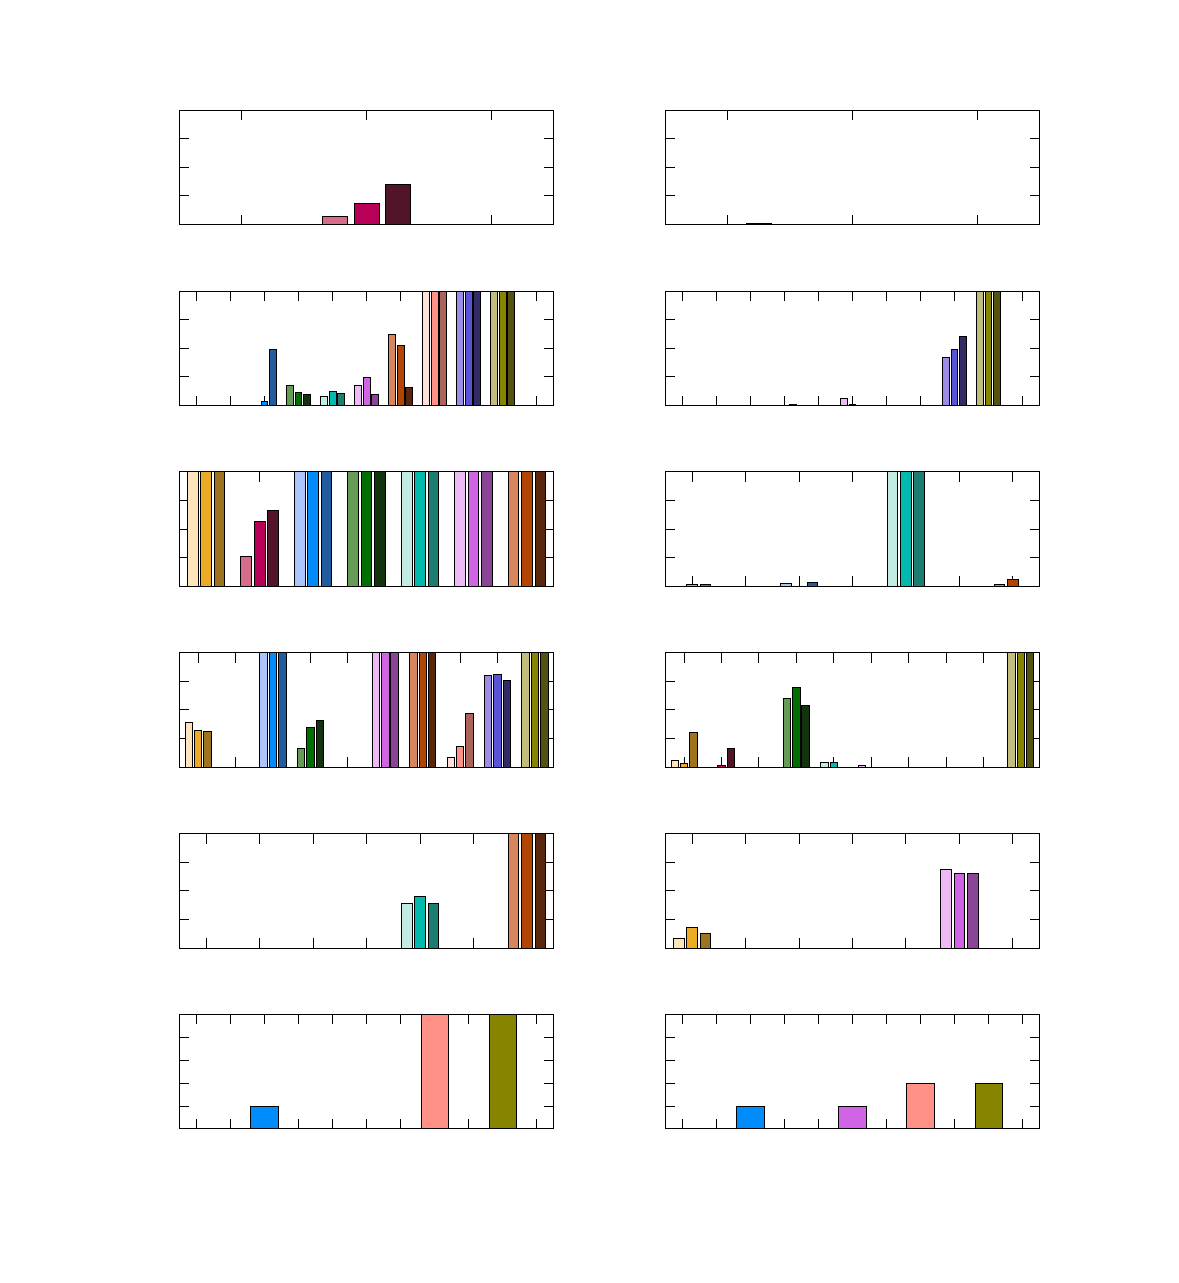
\includegraphics{./figures/parts/02/chapters/03/sections/04/outliers}}%
    \gplfronttext
  \end{picture}%
\endgroup

\caption{}
\label{}
\end{figure}

\begin{figure}
  \hspace{-1cm}
  \begin{subfigure}{0.5\linewidth}
    % GNUPLOT: LaTeX picture with Postscript
\begingroup
  \makeatletter
  \providecommand\color[2][]{%
    \GenericError{(gnuplot) \space\space\space\@spaces}{%
      Package color not loaded in conjunction with
      terminal option `colourtext'%
    }{See the gnuplot documentation for explanation.%
    }{Either use 'blacktext' in gnuplot or load the package
      color.sty in LaTeX.}%
    \renewcommand\color[2][]{}%
  }%
  \providecommand\includegraphics[2][]{%
    \GenericError{(gnuplot) \space\space\space\@spaces}{%
      Package graphicx or graphics not loaded%
    }{See the gnuplot documentation for explanation.%
    }{The gnuplot epslatex terminal needs graphicx.sty or graphics.sty.}%
    \renewcommand\includegraphics[2][]{}%
  }%
  \providecommand\rotatebox[2]{#2}%
  \@ifundefined{ifGPcolor}{%
    \newif\ifGPcolor
    \GPcolorfalse
  }{}%
  \@ifundefined{ifGPblacktext}{%
    \newif\ifGPblacktext
    \GPblacktexttrue
  }{}%
  % define a \g@addto@macro without @ in the name:
  \let\gplgaddtomacro\g@addto@macro
  % define empty templates for all commands taking text:
  \gdef\gplfronttext{}%
  \gdef\gplfronttext{}%
  \makeatother
  \ifGPblacktext
    % no textcolor at all
    \def\colorrgb#1{}%
    \def\colorgray#1{}%
  \else
    % gray or color?
    \ifGPcolor
      \def\colorrgb#1{\color[rgb]{#1}}%
      \def\colorgray#1{\color[gray]{#1}}%
      \expandafter\def\csname LTw\endcsname{\color{white}}%
      \expandafter\def\csname LTb\endcsname{\color{black}}%
      \expandafter\def\csname LTa\endcsname{\color{black}}%
      \expandafter\def\csname LT0\endcsname{\color[rgb]{1,0,0}}%
      \expandafter\def\csname LT1\endcsname{\color[rgb]{0,1,0}}%
      \expandafter\def\csname LT2\endcsname{\color[rgb]{0,0,1}}%
      \expandafter\def\csname LT3\endcsname{\color[rgb]{1,0,1}}%
      \expandafter\def\csname LT4\endcsname{\color[rgb]{0,1,1}}%
      \expandafter\def\csname LT5\endcsname{\color[rgb]{1,1,0}}%
      \expandafter\def\csname LT6\endcsname{\color[rgb]{0,0,0}}%
      \expandafter\def\csname LT7\endcsname{\color[rgb]{1,0.3,0}}%
      \expandafter\def\csname LT8\endcsname{\color[rgb]{0.5,0.5,0.5}}%
    \else
      % gray
      \def\colorrgb#1{\color{black}}%
      \def\colorgray#1{\color[gray]{#1}}%
      \expandafter\def\csname LTw\endcsname{\color{white}}%
      \expandafter\def\csname LTb\endcsname{\color{black}}%
      \expandafter\def\csname LTa\endcsname{\color{black}}%
      \expandafter\def\csname LT0\endcsname{\color{black}}%
      \expandafter\def\csname LT1\endcsname{\color{black}}%
      \expandafter\def\csname LT2\endcsname{\color{black}}%
      \expandafter\def\csname LT3\endcsname{\color{black}}%
      \expandafter\def\csname LT4\endcsname{\color{black}}%
      \expandafter\def\csname LT5\endcsname{\color{black}}%
      \expandafter\def\csname LT6\endcsname{\color{black}}%
      \expandafter\def\csname LT7\endcsname{\color{black}}%
      \expandafter\def\csname LT8\endcsname{\color{black}}%
    \fi
  \fi
  \setlength{\unitlength}{0.0500bp}%
  \begin{picture}(4800.00,12000.00)%
    \gplgaddtomacro\gplfronttext{%
      \colorrgb{0.00,0.00,0.00}%
      \put(492,9720){\makebox(0,0)[r]{\strut{}\small $0.0$}}%
      \colorrgb{0.00,0.00,0.00}%
      \put(492,9996){\makebox(0,0)[r]{\strut{}\small $0.01$}}%
      \colorrgb{0.00,0.00,0.00}%
      \put(492,10272){\makebox(0,0)[r]{\strut{}\small $0.02$}}%
      \colorrgb{0.00,0.00,0.00}%
      \put(492,10547){\makebox(0,0)[r]{\strut{}\small $0.03$}}%
      \colorrgb{0.00,0.00,0.00}%
      \put(492,10823){\makebox(0,0)[r]{\strut{}\small $0.04$}}%
      \colorrgb{0.00,0.00,0.00}%
      \put(492,11099){\makebox(0,0)[r]{\strut{}\small $0.05$}}%
      \colorrgb{0.00,0.00,0.00}%
      \put(874,9500){\makebox(0,0){\strut{}}}%
      \colorrgb{0.00,0.00,0.00}%
      \put(1374,9500){\makebox(0,0){\strut{}}}%
      \colorrgb{0.00,0.00,0.00}%
      \put(1873,9500){\makebox(0,0){\strut{}}}%
      \colorrgb{0.00,0.00,0.00}%
      \put(-342,10409){\rotatebox{90}{\makebox(0,0){\strut{}\small CORRIDOR}}}%
      \colorrgb{0.00,0.00,0.00}%
      \put(1373,11429){\makebox(0,0){\strut{}PLICP}}%
    }%
    \gplgaddtomacro\gplfronttext{%
    }%
    \gplgaddtomacro\gplfronttext{%
      \colorrgb{0.00,0.00,0.00}%
      \put(2712,9720){\makebox(0,0)[r]{\strut{}\small $0.0$}}%
      \colorrgb{0.00,0.00,0.00}%
      \put(2712,9996){\makebox(0,0)[r]{\strut{}\small $0.01$}}%
      \colorrgb{0.00,0.00,0.00}%
      \put(2712,10272){\makebox(0,0)[r]{\strut{}\small $0.02$}}%
      \colorrgb{0.00,0.00,0.00}%
      \put(2712,10547){\makebox(0,0)[r]{\strut{}\small $0.03$}}%
      \colorrgb{0.00,0.00,0.00}%
      \put(2712,10823){\makebox(0,0)[r]{\strut{}\small $0.04$}}%
      \colorrgb{0.00,0.00,0.00}%
      \put(2712,11099){\makebox(0,0)[r]{\strut{}\small $0.05$}}%
      \colorrgb{0.00,0.00,0.00}%
      \put(3094,9500){\makebox(0,0){\strut{}}}%
      \colorrgb{0.00,0.00,0.00}%
      \put(3594,9500){\makebox(0,0){\strut{}}}%
      \colorrgb{0.00,0.00,0.00}%
      \put(4093,9500){\makebox(0,0){\strut{}}}%
      \colorrgb{0.00,0.00,0.00}%
      \put(3593,11429){\makebox(0,0){\strut{}PGL-FMIC}}%
    }%
    \gplgaddtomacro\gplfronttext{%
    }%
    \gplgaddtomacro\gplfronttext{%
      \colorrgb{0.00,0.00,0.00}%
      \put(492,7830){\makebox(0,0)[r]{\strut{}\small $0.0$}}%
      \colorrgb{0.00,0.00,0.00}%
      \put(492,8106){\makebox(0,0)[r]{\strut{}\small $0.05$}}%
      \colorrgb{0.00,0.00,0.00}%
      \put(492,8382){\makebox(0,0)[r]{\strut{}\small $0.10$}}%
      \colorrgb{0.00,0.00,0.00}%
      \put(492,8657){\makebox(0,0)[r]{\strut{}\small $0.15$}}%
      \colorrgb{0.00,0.00,0.00}%
      \put(492,8933){\makebox(0,0)[r]{\strut{}\small $0.20$}}%
      \colorrgb{0.00,0.00,0.00}%
      \put(492,9209){\makebox(0,0)[r]{\strut{}\small $0.25$}}%
      \colorrgb{0.00,0.00,0.00}%
      \put(874,7610){\makebox(0,0){\strut{}}}%
      \colorrgb{0.00,0.00,0.00}%
      \put(1374,7610){\makebox(0,0){\strut{}}}%
      \colorrgb{0.00,0.00,0.00}%
      \put(1873,7610){\makebox(0,0){\strut{}}}%
      \colorrgb{0.00,0.00,0.00}%
      \put(-342,8519){\rotatebox{90}{\makebox(0,0){\strut{}\small HOME}}}%
    }%
    \gplgaddtomacro\gplfronttext{%
    }%
    \gplgaddtomacro\gplfronttext{%
      \colorrgb{0.00,0.00,0.00}%
      \put(2712,7830){\makebox(0,0)[r]{\strut{}\small $0.0$}}%
      \colorrgb{0.00,0.00,0.00}%
      \put(2712,8106){\makebox(0,0)[r]{\strut{}\small $0.05$}}%
      \colorrgb{0.00,0.00,0.00}%
      \put(2712,8382){\makebox(0,0)[r]{\strut{}\small $0.10$}}%
      \colorrgb{0.00,0.00,0.00}%
      \put(2712,8657){\makebox(0,0)[r]{\strut{}\small $0.15$}}%
      \colorrgb{0.00,0.00,0.00}%
      \put(2712,8933){\makebox(0,0)[r]{\strut{}\small $0.20$}}%
      \colorrgb{0.00,0.00,0.00}%
      \put(2712,9209){\makebox(0,0)[r]{\strut{}\small $0.25$}}%
      \colorrgb{0.00,0.00,0.00}%
      \put(3094,7610){\makebox(0,0){\strut{}}}%
      \colorrgb{0.00,0.00,0.00}%
      \put(3594,7610){\makebox(0,0){\strut{}}}%
      \colorrgb{0.00,0.00,0.00}%
      \put(4093,7610){\makebox(0,0){\strut{}}}%
    }%
    \gplgaddtomacro\gplfronttext{%
    }%
    \gplgaddtomacro\gplfronttext{%
      \colorrgb{0.00,0.00,0.00}%
      \put(492,5940){\makebox(0,0)[r]{\strut{}\small $3.14$}}%
      \colorrgb{0.00,0.00,0.00}%
      \put(492,7319){\makebox(0,0)[r]{\strut{}\small $3.26$}}%
      \colorrgb{0.00,0.00,0.00}%
      \put(874,5720){\makebox(0,0){\strut{}}}%
      \colorrgb{0.00,0.00,0.00}%
      \put(1374,5720){\makebox(0,0){\strut{}}}%
      \colorrgb{0.00,0.00,0.00}%
      \put(1873,5720){\makebox(0,0){\strut{}}}%
      \colorrgb{0.00,0.00,0.00}%
      \put(-342,6629){\rotatebox{90}{\makebox(0,0){\strut{}\small WAREHOUSE}}}%
    }%
    \gplgaddtomacro\gplfronttext{%
    }%
    \gplgaddtomacro\gplfronttext{%
      \colorrgb{0.00,0.00,0.00}%
      \put(2712,5940){\makebox(0,0)[r]{\strut{}\small $0.04$}}%
      \colorrgb{0.00,0.00,0.00}%
      \put(2712,6170){\makebox(0,0)[r]{\strut{}\small $0.06$}}%
      \colorrgb{0.00,0.00,0.00}%
      \put(2712,6400){\makebox(0,0)[r]{\strut{}\small $0.08$}}%
      \colorrgb{0.00,0.00,0.00}%
      \put(2712,6630){\makebox(0,0)[r]{\strut{}\small $0.10$}}%
      \colorrgb{0.00,0.00,0.00}%
      \put(2712,6859){\makebox(0,0)[r]{\strut{}\small $0.12$}}%
      \colorrgb{0.00,0.00,0.00}%
      \put(2712,7089){\makebox(0,0)[r]{\strut{}\small $0.14$}}%
      \colorrgb{0.00,0.00,0.00}%
      \put(2712,7319){\makebox(0,0)[r]{\strut{}\small $0.16$}}%
      \colorrgb{0.00,0.00,0.00}%
      \put(3094,5720){\makebox(0,0){\strut{}}}%
      \colorrgb{0.00,0.00,0.00}%
      \put(3594,5720){\makebox(0,0){\strut{}}}%
      \colorrgb{0.00,0.00,0.00}%
      \put(4093,5720){\makebox(0,0){\strut{}}}%
    }%
    \gplgaddtomacro\gplfronttext{%
    }%
    \gplgaddtomacro\gplfronttext{%
      \colorrgb{0.00,0.00,0.00}%
      \put(492,4050){\makebox(0,0)[r]{\strut{}\small $0.0$}}%
      \colorrgb{0.00,0.00,0.00}%
      \put(492,4346){\makebox(0,0)[r]{\strut{}\small $0.30$}}%
      \colorrgb{0.00,0.00,0.00}%
      \put(492,4641){\makebox(0,0)[r]{\strut{}\small $0.60$}}%
      \colorrgb{0.00,0.00,0.00}%
      \put(492,4937){\makebox(0,0)[r]{\strut{}\small $0.90$}}%
      \colorrgb{0.00,0.00,0.00}%
      \put(492,5232){\makebox(0,0)[r]{\strut{}\small $1.2$}}%
      \colorrgb{0.00,0.00,0.00}%
      \put(874,3830){\makebox(0,0){\strut{}}}%
      \colorrgb{0.00,0.00,0.00}%
      \put(1374,3830){\makebox(0,0){\strut{}}}%
      \colorrgb{0.00,0.00,0.00}%
      \put(1873,3830){\makebox(0,0){\strut{}}}%
      \colorrgb{0.00,0.00,0.00}%
      \put(-342,4739){\rotatebox{90}{\makebox(0,0){\strut{}\small WILLOWGARAGE}}}%
    }%
    \gplgaddtomacro\gplfronttext{%
    }%
    \gplgaddtomacro\gplfronttext{%
      \colorrgb{0.00,0.00,0.00}%
      \put(2712,4050){\makebox(0,0)[r]{\strut{}\small $0.0$}}%
      \colorrgb{0.00,0.00,0.00}%
      \put(2712,4444){\makebox(0,0)[r]{\strut{}\small $0.10$}}%
      \colorrgb{0.00,0.00,0.00}%
      \put(2712,4838){\makebox(0,0)[r]{\strut{}\small $0.20$}}%
      \colorrgb{0.00,0.00,0.00}%
      \put(2712,5232){\makebox(0,0)[r]{\strut{}\small $0.30$}}%
      \colorrgb{0.00,0.00,0.00}%
      \put(3094,3830){\makebox(0,0){\strut{}}}%
      \colorrgb{0.00,0.00,0.00}%
      \put(3594,3830){\makebox(0,0){\strut{}}}%
      \colorrgb{0.00,0.00,0.00}%
      \put(4093,3830){\makebox(0,0){\strut{}}}%
    }%
    \gplgaddtomacro\gplfronttext{%
    }%
    \gplgaddtomacro\gplfronttext{%
      \colorrgb{0.00,0.00,0.00}%
      \put(492,2160){\makebox(0,0)[r]{\strut{}\small $0.25$}}%
      \colorrgb{0.00,0.00,0.00}%
      \put(492,2505){\makebox(0,0)[r]{\strut{}\small $0.30$}}%
      \colorrgb{0.00,0.00,0.00}%
      \put(492,2850){\makebox(0,0)[r]{\strut{}\small $0.35$}}%
      \colorrgb{0.00,0.00,0.00}%
      \put(492,3194){\makebox(0,0)[r]{\strut{}\small $0.40$}}%
      \colorrgb{0.00,0.00,0.00}%
      \put(492,3539){\makebox(0,0)[r]{\strut{}\small $0.45$}}%
      \colorrgb{0.00,0.00,0.00}%
      \put(874,1940){\makebox(0,0){\strut{}\scriptsize $0.01$}}%
      \colorrgb{0.00,0.00,0.00}%
      \put(1374,1940){\makebox(0,0){\strut{}\scriptsize  $0.02$}}%
      \colorrgb{0.00,0.00,0.00}%
      \put(1873,1940){\makebox(0,0){\strut{}\scriptsize  $0.05$}}%
      \colorrgb{0.00,0.00,0.00}%
      \put(-342,2849){\rotatebox{90}{\makebox(0,0){\strut{}\small LANDFILL}}}%
    }%
    \gplgaddtomacro\gplfronttext{%
    }%
    \gplgaddtomacro\gplfronttext{%
      \colorrgb{0.00,0.00,0.00}%
      \put(2712,2160){\makebox(0,0)[r]{\strut{}\small $0.25$}}%
      \colorrgb{0.00,0.00,0.00}%
      \put(2712,2505){\makebox(0,0)[r]{\strut{}\small $0.30$}}%
      \colorrgb{0.00,0.00,0.00}%
      \put(2712,2850){\makebox(0,0)[r]{\strut{}\small $0.35$}}%
      \colorrgb{0.00,0.00,0.00}%
      \put(2712,3194){\makebox(0,0)[r]{\strut{}\small $0.40$}}%
      \colorrgb{0.00,0.00,0.00}%
      \put(2712,3539){\makebox(0,0)[r]{\strut{}\small $0.45$}}%
      \colorrgb{0.00,0.00,0.00}%
      \put(3094,1940){\makebox(0,0){\strut{}\scriptsize  $0.01$}}%
      \colorrgb{0.00,0.00,0.00}%
      \put(3594,1940){\makebox(0,0){\strut{}\scriptsize  $0.02$}}%
      \colorrgb{0.00,0.00,0.00}%
      \put(4093,1940){\makebox(0,0){\strut{}\scriptsize  $0.05$}}%
      \colorrgb{0.00,0.00,0.00}%
      \put(2500,1610){\makebox(0,0){\strut{}\small $d$ [m]: Θόρυβος μέτρησης $\mathcal{N}(0.0,d)$}}%
    }%
    \gplgaddtomacro\gplfronttext{%
    }%
    \put(0,0){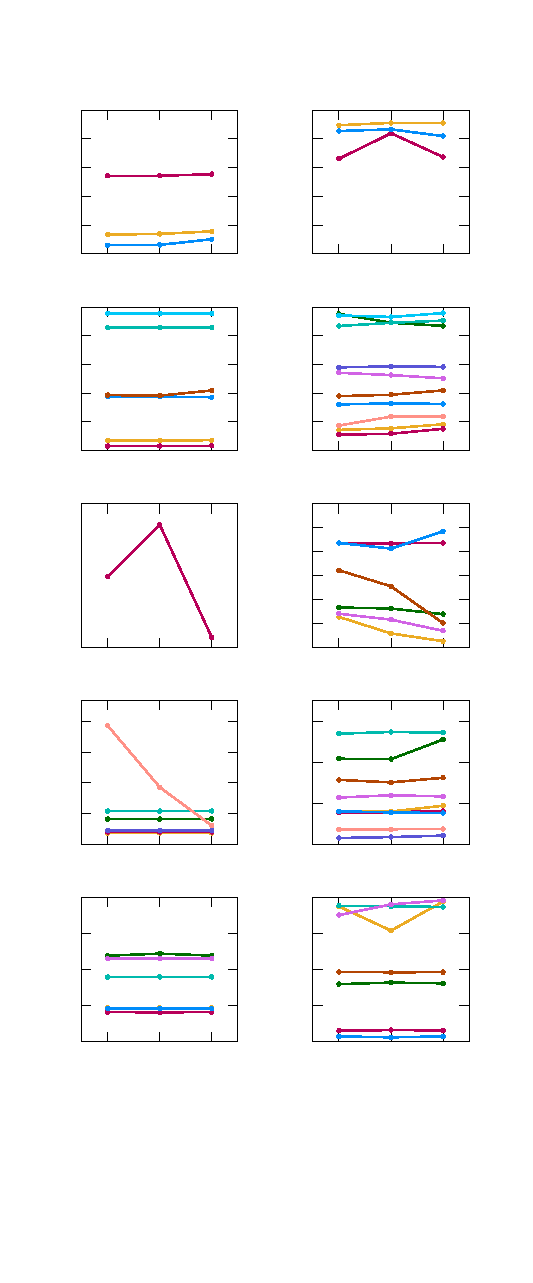
\includegraphics{./figures/parts/02/chapters/03/sections/04/simulations_pose_errors}}%
    \gplfronttext
  \end{picture}%
\endgroup

    \caption{}
    \label{}
  \end{subfigure}\hspace{1.0cm}
  \begin{subfigure}{0.5\linewidth}
    % GNUPLOT: LaTeX picture with Postscript
\begingroup
  \makeatletter
  \providecommand\color[2][]{%
    \GenericError{(gnuplot) \space\space\space\@spaces}{%
      Package color not loaded in conjunction with
      terminal option `colourtext'%
    }{See the gnuplot documentation for explanation.%
    }{Either use 'blacktext' in gnuplot or load the package
      color.sty in LaTeX.}%
    \renewcommand\color[2][]{}%
  }%
  \providecommand\includegraphics[2][]{%
    \GenericError{(gnuplot) \space\space\space\@spaces}{%
      Package graphicx or graphics not loaded%
    }{See the gnuplot documentation for explanation.%
    }{The gnuplot epslatex terminal needs graphicx.sty or graphics.sty.}%
    \renewcommand\includegraphics[2][]{}%
  }%
  \providecommand\rotatebox[2]{#2}%
  \@ifundefined{ifGPcolor}{%
    \newif\ifGPcolor
    \GPcolorfalse
  }{}%
  \@ifundefined{ifGPblacktext}{%
    \newif\ifGPblacktext
    \GPblacktexttrue
  }{}%
  % define a \g@addto@macro without @ in the name:
  \let\gplgaddtomacro\g@addto@macro
  % define empty templates for all commands taking text:
  \gdef\gplfronttext{}%
  \gdef\gplfronttext{}%
  \makeatother
  \ifGPblacktext
    % no textcolor at all
    \def\colorrgb#1{}%
    \def\colorgray#1{}%
  \else
    % gray or color?
    \ifGPcolor
      \def\colorrgb#1{\color[rgb]{#1}}%
      \def\colorgray#1{\color[gray]{#1}}%
      \expandafter\def\csname LTw\endcsname{\color{white}}%
      \expandafter\def\csname LTb\endcsname{\color{black}}%
      \expandafter\def\csname LTa\endcsname{\color{black}}%
      \expandafter\def\csname LT0\endcsname{\color[rgb]{1,0,0}}%
      \expandafter\def\csname LT1\endcsname{\color[rgb]{0,1,0}}%
      \expandafter\def\csname LT2\endcsname{\color[rgb]{0,0,1}}%
      \expandafter\def\csname LT3\endcsname{\color[rgb]{1,0,1}}%
      \expandafter\def\csname LT4\endcsname{\color[rgb]{0,1,1}}%
      \expandafter\def\csname LT5\endcsname{\color[rgb]{1,1,0}}%
      \expandafter\def\csname LT6\endcsname{\color[rgb]{0,0,0}}%
      \expandafter\def\csname LT7\endcsname{\color[rgb]{1,0.3,0}}%
      \expandafter\def\csname LT8\endcsname{\color[rgb]{0.5,0.5,0.5}}%
    \else
      % gray
      \def\colorrgb#1{\color{black}}%
      \def\colorgray#1{\color[gray]{#1}}%
      \expandafter\def\csname LTw\endcsname{\color{white}}%
      \expandafter\def\csname LTb\endcsname{\color{black}}%
      \expandafter\def\csname LTa\endcsname{\color{black}}%
      \expandafter\def\csname LT0\endcsname{\color{black}}%
      \expandafter\def\csname LT1\endcsname{\color{black}}%
      \expandafter\def\csname LT2\endcsname{\color{black}}%
      \expandafter\def\csname LT3\endcsname{\color{black}}%
      \expandafter\def\csname LT4\endcsname{\color{black}}%
      \expandafter\def\csname LT5\endcsname{\color{black}}%
      \expandafter\def\csname LT6\endcsname{\color{black}}%
      \expandafter\def\csname LT7\endcsname{\color{black}}%
      \expandafter\def\csname LT8\endcsname{\color{black}}%
    \fi
  \fi
  \setlength{\unitlength}{0.0500bp}%
  \begin{picture}(4800.00,12000.00)%
    \gplgaddtomacro\gplfronttext{%
      \colorrgb{0.00,0.00,0.00}%
      \put(492,9720){\makebox(0,0)[r]{\strut{}\small $160$}}%
      \colorrgb{0.00,0.00,0.00}%
      \put(492,10065){\makebox(0,0)[r]{\strut{}\small $200$}}%
      \colorrgb{0.00,0.00,0.00}%
      \put(492,10410){\makebox(0,0)[r]{\strut{}\small $240$}}%
      \colorrgb{0.00,0.00,0.00}%
      \put(492,10754){\makebox(0,0)[r]{\strut{}\small $280$}}%
      \colorrgb{0.00,0.00,0.00}%
      \put(492,11099){\makebox(0,0)[r]{\strut{}\small $320$}}%
      \colorrgb{0.00,0.00,0.00}%
      \put(874,9500){\makebox(0,0){\strut{}}}%
      \colorrgb{0.00,0.00,0.00}%
      \put(1374,9500){\makebox(0,0){\strut{}}}%
      \colorrgb{0.00,0.00,0.00}%
      \put(1873,9500){\makebox(0,0){\strut{}}}%
      \colorrgb{0.00,0.00,0.00}%
      %\put(-410,10409){\rotatebox{90}{\makebox(0,0){\strut{}\small CORRIDOR}}}%
      \colorrgb{0.00,0.00,0.00}%
      \put(1373,11429){\makebox(0,0){\strut{}PLICP}}%
      \put(2500,11829){\makebox(0,0){\strut{}Χρόνος εκτέλεσης [ms]}}%
    }%
    \gplgaddtomacro\gplfronttext{%
    }%
    \gplgaddtomacro\gplfronttext{%
      \colorrgb{0.00,0.00,0.00}%
      \put(2712,9720){\makebox(0,0)[r]{\strut{}\small $160$}}%
      \colorrgb{0.00,0.00,0.00}%
      \put(2712,10065){\makebox(0,0)[r]{\strut{}\small $200$}}%
      \colorrgb{0.00,0.00,0.00}%
      \put(2712,10410){\makebox(0,0)[r]{\strut{}\small $240$}}%
      \colorrgb{0.00,0.00,0.00}%
      \put(2712,10754){\makebox(0,0)[r]{\strut{}\small $208$}}%
      \colorrgb{0.00,0.00,0.00}%
      \put(2712,11099){\makebox(0,0)[r]{\strut{}\small $320$}}%
      \colorrgb{0.00,0.00,0.00}%
      \put(3094,9500){\makebox(0,0){\strut{}}}%
      \colorrgb{0.00,0.00,0.00}%
      \put(3594,9500){\makebox(0,0){\strut{}}}%
      \colorrgb{0.00,0.00,0.00}%
      \put(4093,9500){\makebox(0,0){\strut{}}}%
      \colorrgb{0.00,0.00,0.00}%
      \put(3593,11429){\makebox(0,0){\strut{}PGL-FMIC}}%
    }%
    \gplgaddtomacro\gplfronttext{%
    }%
    \gplgaddtomacro\gplfronttext{%
      \colorrgb{0.00,0.00,0.00}%
      \put(492,7830){\makebox(0,0)[r]{\strut{}\small $160$}}%
      \colorrgb{0.00,0.00,0.00}%
      \put(492,8175){\makebox(0,0)[r]{\strut{}\small $240$}}%
      \colorrgb{0.00,0.00,0.00}%
      \put(492,8520){\makebox(0,0)[r]{\strut{}\small $320$}}%
      \colorrgb{0.00,0.00,0.00}%
      \put(492,8864){\makebox(0,0)[r]{\strut{}\small $400$}}%
      \colorrgb{0.00,0.00,0.00}%
      \put(492,9209){\makebox(0,0)[r]{\strut{}\small $480$}}%
      \colorrgb{0.00,0.00,0.00}%
      \put(874,7610){\makebox(0,0){\strut{}}}%
      \colorrgb{0.00,0.00,0.00}%
      \put(1374,7610){\makebox(0,0){\strut{}}}%
      \colorrgb{0.00,0.00,0.00}%
      \put(1873,7610){\makebox(0,0){\strut{}}}%
      \colorrgb{0.00,0.00,0.00}%
      %\put(-410,8519){\rotatebox{90}{\makebox(0,0){\strut{}\small HOME}}}%
    }%
    \gplgaddtomacro\gplfronttext{%
    }%
    \gplgaddtomacro\gplfronttext{%
      \colorrgb{0.00,0.00,0.00}%
      \put(2712,7830){\makebox(0,0)[r]{\strut{}\small $160$}}%
      \colorrgb{0.00,0.00,0.00}%
      \put(2712,8175){\makebox(0,0)[r]{\strut{}\small $240$}}%
      \colorrgb{0.00,0.00,0.00}%
      \put(2712,8520){\makebox(0,0)[r]{\strut{}\small $320$}}%
      \colorrgb{0.00,0.00,0.00}%
      \put(2712,8864){\makebox(0,0)[r]{\strut{}\small $400$}}%
      \colorrgb{0.00,0.00,0.00}%
      \put(2712,9209){\makebox(0,0)[r]{\strut{}\small $480$}}%
      \colorrgb{0.00,0.00,0.00}%
      \put(3094,7610){\makebox(0,0){\strut{}}}%
      \colorrgb{0.00,0.00,0.00}%
      \put(3594,7610){\makebox(0,0){\strut{}}}%
      \colorrgb{0.00,0.00,0.00}%
      \put(4093,7610){\makebox(0,0){\strut{}}}%
    }%
    \gplgaddtomacro\gplfronttext{%
    }%
    \gplgaddtomacro\gplfronttext{%
      \colorrgb{0.00,0.00,0.00}%
      \put(492,5940){\makebox(0,0)[r]{\strut{}\small $200$}}%
      \colorrgb{0.00,0.00,0.00}%
      \put(492,6400){\makebox(0,0)[r]{\strut{}\small $280$}}%
      \colorrgb{0.00,0.00,0.00}%
      \put(492,6859){\makebox(0,0)[r]{\strut{}\small $360$}}%
      \colorrgb{0.00,0.00,0.00}%
      \put(492,7319){\makebox(0,0)[r]{\strut{}\small $440$}}%
      \colorrgb{0.00,0.00,0.00}%
      \put(874,5720){\makebox(0,0){\strut{}}}%
      \colorrgb{0.00,0.00,0.00}%
      \put(1374,5720){\makebox(0,0){\strut{}}}%
      \colorrgb{0.00,0.00,0.00}%
      \put(1873,5720){\makebox(0,0){\strut{}}}%
      \colorrgb{0.00,0.00,0.00}%
      %\put(-410,6629){\rotatebox{90}{\makebox(0,0){\strut{}\small WAREHOUSE}}}%
    }%
    \gplgaddtomacro\gplfronttext{%
    }%
    \gplgaddtomacro\gplfronttext{%
      \colorrgb{0.00,0.00,0.00}%
      \put(2712,5940){\makebox(0,0)[r]{\strut{}\small $200$}}%
      \colorrgb{0.00,0.00,0.00}%
      \put(2712,6400){\makebox(0,0)[r]{\strut{}\small $280$}}%
      \colorrgb{0.00,0.00,0.00}%
      \put(2712,6859){\makebox(0,0)[r]{\strut{}\small $360$}}%
      \colorrgb{0.00,0.00,0.00}%
      \put(2712,7319){\makebox(0,0)[r]{\strut{}\small $440$}}%
      \colorrgb{0.00,0.00,0.00}%
      \put(3094,5720){\makebox(0,0){\strut{}}}%
      \colorrgb{0.00,0.00,0.00}%
      \put(3594,5720){\makebox(0,0){\strut{}}}%
      \colorrgb{0.00,0.00,0.00}%
      \put(4093,5720){\makebox(0,0){\strut{}}}%
    }%
    \gplgaddtomacro\gplfronttext{%
    }%
    \gplgaddtomacro\gplfronttext{%
      \colorrgb{0.00,0.00,0.00}%
      \put(492,4050){\makebox(0,0)[r]{\strut{}\small $50$}}%
      \colorrgb{0.00,0.00,0.00}%
      \put(492,4247){\makebox(0,0)[r]{\strut{}\small $100$}}%
      \colorrgb{0.00,0.00,0.00}%
      \put(492,4444){\makebox(0,0)[r]{\strut{}\small $150$}}%
      \colorrgb{0.00,0.00,0.00}%
      \put(492,4641){\makebox(0,0)[r]{\strut{}\small $200$}}%
      \colorrgb{0.00,0.00,0.00}%
      \put(492,4838){\makebox(0,0)[r]{\strut{}\small $250$}}%
      \colorrgb{0.00,0.00,0.00}%
      \put(492,5035){\makebox(0,0)[r]{\strut{}\small $300$}}%
      \colorrgb{0.00,0.00,0.00}%
      \put(492,5232){\makebox(0,0)[r]{\strut{}\small $350$}}%
      \colorrgb{0.00,0.00,0.00}%
      \put(492,5429){\makebox(0,0)[r]{\strut{}\small $400$}}%
      \colorrgb{0.00,0.00,0.00}%
      \put(874,3830){\makebox(0,0){\strut{}}}%
      \colorrgb{0.00,0.00,0.00}%
      \put(1374,3830){\makebox(0,0){\strut{}}}%
      \colorrgb{0.00,0.00,0.00}%
      \put(1873,3830){\makebox(0,0){\strut{}}}%
      \colorrgb{0.00,0.00,0.00}%
      %\put(-410,4739){\rotatebox{90}{\makebox(0,0){\strut{}\small WILLOWGARAGE}}}%
    }%
    \gplgaddtomacro\gplfronttext{%
    }%
    \gplgaddtomacro\gplfronttext{%
      \colorrgb{0.00,0.00,0.00}%
      \put(2712,4050){\makebox(0,0)[r]{\strut{}\small $50$}}%
      \colorrgb{0.00,0.00,0.00}%
      \put(2712,4247){\makebox(0,0)[r]{\strut{}\small $100$}}%
      \colorrgb{0.00,0.00,0.00}%
      \put(2712,4444){\makebox(0,0)[r]{\strut{}\small $150$}}%
      \colorrgb{0.00,0.00,0.00}%
      \put(2712,4641){\makebox(0,0)[r]{\strut{}\small $200$}}%
      \colorrgb{0.00,0.00,0.00}%
      \put(2712,4838){\makebox(0,0)[r]{\strut{}\small $250$}}%
      \colorrgb{0.00,0.00,0.00}%
      \put(2712,5035){\makebox(0,0)[r]{\strut{}\small $300$}}%
      \colorrgb{0.00,0.00,0.00}%
      \put(2712,5232){\makebox(0,0)[r]{\strut{}\small $350$}}%
      \colorrgb{0.00,0.00,0.00}%
      \put(2712,5429){\makebox(0,0)[r]{\strut{}\small $400$}}%
      \colorrgb{0.00,0.00,0.00}%
      \put(3094,3830){\makebox(0,0){\strut{}}}%
      \colorrgb{0.00,0.00,0.00}%
      \put(3594,3830){\makebox(0,0){\strut{}}}%
      \colorrgb{0.00,0.00,0.00}%
      \put(4093,3830){\makebox(0,0){\strut{}}}%
    }%
    \gplgaddtomacro\gplfronttext{%
    }%
    \gplgaddtomacro\gplfronttext{%
      \colorrgb{0.00,0.00,0.00}%
      \put(492,2160){\makebox(0,0)[r]{\strut{}\small $200$}}%
      \colorrgb{0.00,0.00,0.00}%
      \put(492,2620){\makebox(0,0)[r]{\strut{}\small $250$}}%
      \colorrgb{0.00,0.00,0.00}%
      \put(492,3079){\makebox(0,0)[r]{\strut{}\small $300$}}%
      \colorrgb{0.00,0.00,0.00}%
      \put(492,3539){\makebox(0,0)[r]{\strut{}\small $350$}}%
      \colorrgb{0.00,0.00,0.00}%
      \put(874,1940){\makebox(0,0){\strut{}\scriptsize  $0.01$}}%
      \colorrgb{0.00,0.00,0.00}%
      \put(1374,1940){\makebox(0,0){\strut{}\scriptsize  $0.02$}}%
      \colorrgb{0.00,0.00,0.00}%
      \put(1873,1940){\makebox(0,0){\strut{}\scriptsize  $0.05$}}%
      \colorrgb{0.00,0.00,0.00}%
      %\put(-410,2849){\rotatebox{90}{\makebox(0,0){\strut{}\small LANDFILL}}}%
      \colorrgb{0.00,0.00,0.00}%
      \put(2500,1610){\makebox(0,0){\strut{}\small $d$ [m]: Θόρυβος μέτρησης $\mathcal{N}(0.0,d)$}}%
    }%
    \gplgaddtomacro\gplfronttext{%
    }%
    \gplgaddtomacro\gplfronttext{%
      \colorrgb{0.00,0.00,0.00}%
      \put(2712,2160){\makebox(0,0)[r]{\strut{}\small $200$}}%
      \colorrgb{0.00,0.00,0.00}%
      \put(2712,2620){\makebox(0,0)[r]{\strut{}\small $250$}}%
      \colorrgb{0.00,0.00,0.00}%
      \put(2712,3079){\makebox(0,0)[r]{\strut{}\small $300$}}%
      \colorrgb{0.00,0.00,0.00}%
      \put(2712,3539){\makebox(0,0)[r]{\strut{}\small $350$}}%
      \colorrgb{0.00,0.00,0.00}%
      \put(3094,1940){\makebox(0,0){\strut{}\scriptsize $0.01$}}%
      \colorrgb{0.00,0.00,0.00}%
      \put(3594,1940){\makebox(0,0){\strut{}\scriptsize  $0.02$}}%
      \colorrgb{0.00,0.00,0.00}%
      \put(4093,1940){\makebox(0,0){\strut{}\scriptsize  $0.05$}}%
    }%
    \gplgaddtomacro\gplfronttext{%
    }%
    \put(0,0){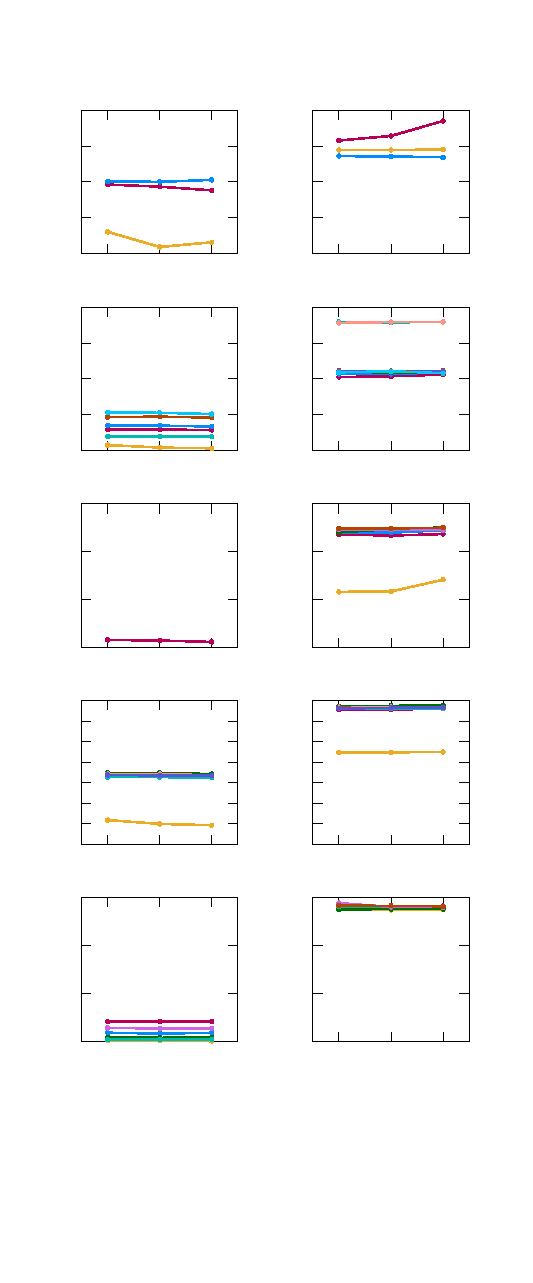
\includegraphics{./figures/parts/02/chapters/03/sections/04/simulations_execution_times}}%
    \gplfronttext
  \end{picture}%
\endgroup

    \caption{}
    \label{}
    \end{subfigure}
\caption{}
\label{}
\end{figure}

\begin{figure}
  \hspace{1cm}
  \begin{subfigure}{0.5\linewidth}
    % GNUPLOT: LaTeX picture with Postscript
\begingroup
  \makeatletter
  \providecommand\color[2][]{%
    \GenericError{(gnuplot) \space\space\space\@spaces}{%
      Package color not loaded in conjunction with
      terminal option `colourtext'%
    }{See the gnuplot documentation for explanation.%
    }{Either use 'blacktext' in gnuplot or load the package
      color.sty in LaTeX.}%
    \renewcommand\color[2][]{}%
  }%
  \providecommand\includegraphics[2][]{%
    \GenericError{(gnuplot) \space\space\space\@spaces}{%
      Package graphicx or graphics not loaded%
    }{See the gnuplot documentation for explanation.%
    }{The gnuplot epslatex terminal needs graphicx.sty or graphics.sty.}%
    \renewcommand\includegraphics[2][]{}%
  }%
  \providecommand\rotatebox[2]{#2}%
  \@ifundefined{ifGPcolor}{%
    \newif\ifGPcolor
    \GPcolorfalse
  }{}%
  \@ifundefined{ifGPblacktext}{%
    \newif\ifGPblacktext
    \GPblacktexttrue
  }{}%
  % define a \g@addto@macro without @ in the name:
  \let\gplgaddtomacro\g@addto@macro
  % define empty templates for all commands taking text:
  \gdef\gplfronttext{}%
  \gdef\gplfronttext{}%
  \makeatother
  \ifGPblacktext
    % no textcolor at all
    \def\colorrgb#1{}%
    \def\colorgray#1{}%
  \else
    % gray or color?
    \ifGPcolor
      \def\colorrgb#1{\color[rgb]{#1}}%
      \def\colorgray#1{\color[gray]{#1}}%
      \expandafter\def\csname LTw\endcsname{\color{white}}%
      \expandafter\def\csname LTb\endcsname{\color{black}}%
      \expandafter\def\csname LTa\endcsname{\color{black}}%
      \expandafter\def\csname LT0\endcsname{\color[rgb]{1,0,0}}%
      \expandafter\def\csname LT1\endcsname{\color[rgb]{0,1,0}}%
      \expandafter\def\csname LT2\endcsname{\color[rgb]{0,0,1}}%
      \expandafter\def\csname LT3\endcsname{\color[rgb]{1,0,1}}%
      \expandafter\def\csname LT4\endcsname{\color[rgb]{0,1,1}}%
      \expandafter\def\csname LT5\endcsname{\color[rgb]{1,1,0}}%
      \expandafter\def\csname LT6\endcsname{\color[rgb]{0,0,0}}%
      \expandafter\def\csname LT7\endcsname{\color[rgb]{1,0.3,0}}%
      \expandafter\def\csname LT8\endcsname{\color[rgb]{0.5,0.5,0.5}}%
    \else
      % gray
      \def\colorrgb#1{\color{black}}%
      \def\colorgray#1{\color[gray]{#1}}%
      \expandafter\def\csname LTw\endcsname{\color{white}}%
      \expandafter\def\csname LTb\endcsname{\color{black}}%
      \expandafter\def\csname LTa\endcsname{\color{black}}%
      \expandafter\def\csname LT0\endcsname{\color{black}}%
      \expandafter\def\csname LT1\endcsname{\color{black}}%
      \expandafter\def\csname LT2\endcsname{\color{black}}%
      \expandafter\def\csname LT3\endcsname{\color{black}}%
      \expandafter\def\csname LT4\endcsname{\color{black}}%
      \expandafter\def\csname LT5\endcsname{\color{black}}%
      \expandafter\def\csname LT6\endcsname{\color{black}}%
      \expandafter\def\csname LT7\endcsname{\color{black}}%
      \expandafter\def\csname LT8\endcsname{\color{black}}%
    \fi
  \fi
  \setlength{\unitlength}{0.0500bp}%
  \begin{picture}(4000.00,3000.00)%
    \gplgaddtomacro\gplfronttext{%
      \colorrgb{0.00,0.00,0.00}%
      \put(388,1822){\makebox(0,0)[r]{\strut{}\small $0.0$}}%
      \colorrgb{0.00,0.00,0.00}%
      \put(388,2060){\makebox(0,0)[r]{\strut{}\small $0.10$}}%
      \colorrgb{0.00,0.00,0.00}%
      \put(388,2298){\makebox(0,0)[r]{\strut{}\small $0.20$}}%
      \colorrgb{0.00,0.00,0.00}%
      \put(388,2536){\makebox(0,0)[r]{\strut{}\small $0.30$}}%
      \colorrgb{0.00,0.00,0.00}%
      \put(388,2774){\makebox(0,0)[r]{\strut{}\small $0.40$}}%
      \colorrgb{0.00,0.00,0.00}%
      \put(778,1602){\makebox(0,0){\strut{}}}%
      \colorrgb{0.00,0.00,0.00}%
      \put(1037,1602){\makebox(0,0){\strut{}}}%
      \colorrgb{0.00,0.00,0.00}%
      \put(1295,1602){\makebox(0,0){\strut{}}}%
      \colorrgb{0.00,0.00,0.00}%
      \put(1553,1602){\makebox(0,0){\strut{}}}%
      \colorrgb{0.00,0.00,0.00}%
      \put(1811,1602){\makebox(0,0){\strut{}}}%
      \colorrgb{0.00,0.00,0.00}%
      \put(2070,1602){\makebox(0,0){\strut{}}}%
      \colorrgb{0.00,0.00,0.00}%
      \put(2328,1602){\makebox(0,0){\strut{}}}%
      \colorrgb{0.00,0.00,0.00}%
      \put(2586,1602){\makebox(0,0){\strut{}}}%
      \colorrgb{0.00,0.00,0.00}%
      \put(2844,1602){\makebox(0,0){\strut{}}}%
      \colorrgb{0.00,0.00,0.00}%
      \put(3103,1602){\makebox(0,0){\strut{}}}%
      \colorrgb{0.00,0.00,0.00}%
      \put(3361,1602){\makebox(0,0){\strut{}}}%
      \colorrgb{0.00,0.00,0.00}%
      \put(-646,2298){\rotatebox{90}{\makebox(0,0){\strut{}PLICP}}}%
      \colorrgb{0.00,0.00,0.00}%
      \put(2069,3104){\makebox(0,0){\strut{}Σφάλμα στάσης}}%
    }%
    \gplgaddtomacro\gplfronttext{%
    }%
    \gplgaddtomacro\gplfronttext{%
      \colorrgb{0.00,0.00,0.00}%
      \put(388,330){\makebox(0,0)[r]{\strut{}\small $0.0$}}%
      \colorrgb{0.00,0.00,0.00}%
      \put(388,568){\makebox(0,0)[r]{\strut{}\small $0.10$}}%
      \colorrgb{0.00,0.00,0.00}%
      \put(388,806){\makebox(0,0)[r]{\strut{}\small $0.20$}}%
      \colorrgb{0.00,0.00,0.00}%
      \put(388,1044){\makebox(0,0)[r]{\strut{}\small $0.30$}}%
      \colorrgb{0.00,0.00,0.00}%
      \put(388,1282){\makebox(0,0)[r]{\strut{}\small $0.40$}}%
      \colorrgb{0.00,0.00,0.00}%
      \put(778,110){\makebox(0,0){\strut{}\small $\bm{p}_a^A$}}%
      \colorrgb{0.00,0.00,0.00}%
      \put(1037,110){\makebox(0,0){\strut{}\small $\bm{p}_b^A$}}%
      \colorrgb{0.00,0.00,0.00}%
      \put(1295,110){\makebox(0,0){\strut{}\small $\bm{p}_c^A$}}%
      \colorrgb{0.00,0.00,0.00}%
      \put(1553,110){\makebox(0,0){\strut{}\small $\bm{p}_d^A$}}%
      \colorrgb{0.00,0.00,0.00}%
      \put(1811,110){\makebox(0,0){\strut{}\small $\bm{p}_e^A$}}%
      \colorrgb{0.00,0.00,0.00}%
      \put(2070,110){\makebox(0,0){\strut{}\small $\bm{p}_f^A$}}%
      \colorrgb{0.00,0.00,0.00}%
      \put(2328,110){\makebox(0,0){\strut{}\small $\bm{p}_g^A$}}%
      \colorrgb{0.00,0.00,0.00}%
      \put(2586,110){\makebox(0,0){\strut{}\small $\bm{p}_h^A$}}%
      \colorrgb{0.00,0.00,0.00}%
      \put(2844,110){\makebox(0,0){\strut{}\small $\bm{p}_i^A$}}%
      \colorrgb{0.00,0.00,0.00}%
      \put(3103,110){\makebox(0,0){\strut{}\small $\bm{p}_j^A$}}%
      \colorrgb{0.00,0.00,0.00}%
      \put(3361,110){\makebox(0,0){\strut{}\small $\bm{p}_k^A$}}%
      \colorrgb{0.00,0.00,0.00}%
      \put(-646,806){\rotatebox{90}{\makebox(0,0){\strut{}PGL-FMIC}}}%
      \colorrgb{0.00,0.00,0.00}%
      \put(2069,-220){\makebox(0,0){\strut{}Σημαίνον στάσης}}%
    }%
    \gplgaddtomacro\gplfronttext{%
    }%
    \put(0,0){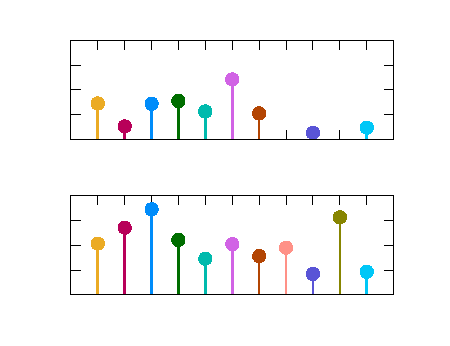
\includegraphics{./figures/parts/02/chapters/03/sections/04/csal_pose_errors}}%
    \gplfronttext
  \end{picture}%
\endgroup

    \caption{}
    \label{}
  \end{subfigure}%
  \begin{subfigure}{0.5\linewidth}
    % GNUPLOT: LaTeX picture with Postscript
\begingroup
  \makeatletter
  \providecommand\color[2][]{%
    \GenericError{(gnuplot) \space\space\space\@spaces}{%
      Package color not loaded in conjunction with
      terminal option `colourtext'%
    }{See the gnuplot documentation for explanation.%
    }{Either use 'blacktext' in gnuplot or load the package
      color.sty in LaTeX.}%
    \renewcommand\color[2][]{}%
  }%
  \providecommand\includegraphics[2][]{%
    \GenericError{(gnuplot) \space\space\space\@spaces}{%
      Package graphicx or graphics not loaded%
    }{See the gnuplot documentation for explanation.%
    }{The gnuplot epslatex terminal needs graphicx.sty or graphics.sty.}%
    \renewcommand\includegraphics[2][]{}%
  }%
  \providecommand\rotatebox[2]{#2}%
  \@ifundefined{ifGPcolor}{%
    \newif\ifGPcolor
    \GPcolorfalse
  }{}%
  \@ifundefined{ifGPblacktext}{%
    \newif\ifGPblacktext
    \GPblacktexttrue
  }{}%
  % define a \g@addto@macro without @ in the name:
  \let\gplgaddtomacro\g@addto@macro
  % define empty templates for all commands taking text:
  \gdef\gplfronttext{}%
  \gdef\gplfronttext{}%
  \makeatother
  \ifGPblacktext
    % no textcolor at all
    \def\colorrgb#1{}%
    \def\colorgray#1{}%
  \else
    % gray or color?
    \ifGPcolor
      \def\colorrgb#1{\color[rgb]{#1}}%
      \def\colorgray#1{\color[gray]{#1}}%
      \expandafter\def\csname LTw\endcsname{\color{white}}%
      \expandafter\def\csname LTb\endcsname{\color{black}}%
      \expandafter\def\csname LTa\endcsname{\color{black}}%
      \expandafter\def\csname LT0\endcsname{\color[rgb]{1,0,0}}%
      \expandafter\def\csname LT1\endcsname{\color[rgb]{0,1,0}}%
      \expandafter\def\csname LT2\endcsname{\color[rgb]{0,0,1}}%
      \expandafter\def\csname LT3\endcsname{\color[rgb]{1,0,1}}%
      \expandafter\def\csname LT4\endcsname{\color[rgb]{0,1,1}}%
      \expandafter\def\csname LT5\endcsname{\color[rgb]{1,1,0}}%
      \expandafter\def\csname LT6\endcsname{\color[rgb]{0,0,0}}%
      \expandafter\def\csname LT7\endcsname{\color[rgb]{1,0.3,0}}%
      \expandafter\def\csname LT8\endcsname{\color[rgb]{0.5,0.5,0.5}}%
    \else
      % gray
      \def\colorrgb#1{\color{black}}%
      \def\colorgray#1{\color[gray]{#1}}%
      \expandafter\def\csname LTw\endcsname{\color{white}}%
      \expandafter\def\csname LTb\endcsname{\color{black}}%
      \expandafter\def\csname LTa\endcsname{\color{black}}%
      \expandafter\def\csname LT0\endcsname{\color{black}}%
      \expandafter\def\csname LT1\endcsname{\color{black}}%
      \expandafter\def\csname LT2\endcsname{\color{black}}%
      \expandafter\def\csname LT3\endcsname{\color{black}}%
      \expandafter\def\csname LT4\endcsname{\color{black}}%
      \expandafter\def\csname LT5\endcsname{\color{black}}%
      \expandafter\def\csname LT6\endcsname{\color{black}}%
      \expandafter\def\csname LT7\endcsname{\color{black}}%
      \expandafter\def\csname LT8\endcsname{\color{black}}%
    \fi
  \fi
  \setlength{\unitlength}{0.0500bp}%
  \begin{picture}(4000.00,3000.00)%
    \gplgaddtomacro\gplfronttext{%
      \colorrgb{0.00,0.00,0.00}%
      \put(388,1822){\makebox(0,0)[r]{\strut{}\small $0$}}%
      \colorrgb{0.00,0.00,0.00}%
      \put(388,1981){\makebox(0,0)[r]{\strut{}\small $200$}}%
      \colorrgb{0.00,0.00,0.00}%
      \put(388,2139){\makebox(0,0)[r]{\strut{}\small $400$}}%
      \colorrgb{0.00,0.00,0.00}%
      \put(388,2298){\makebox(0,0)[r]{\strut{}\small $600$}}%
      \colorrgb{0.00,0.00,0.00}%
      \put(388,2457){\makebox(0,0)[r]{\strut{}\small $800$}}%
      \colorrgb{0.00,0.00,0.00}%
      \put(388,2615){\makebox(0,0)[r]{\strut{}\small $1000$}}%
      \colorrgb{0.00,0.00,0.00}%
      \put(388,2774){\makebox(0,0)[r]{\strut{}\small $1200$}}%
      \colorrgb{0.00,0.00,0.00}%
      \put(778,1602){\makebox(0,0){\strut{}}}%
      \colorrgb{0.00,0.00,0.00}%
      \put(1037,1602){\makebox(0,0){\strut{}}}%
      \colorrgb{0.00,0.00,0.00}%
      \put(1295,1602){\makebox(0,0){\strut{}}}%
      \colorrgb{0.00,0.00,0.00}%
      \put(1553,1602){\makebox(0,0){\strut{}}}%
      \colorrgb{0.00,0.00,0.00}%
      \put(1811,1602){\makebox(0,0){\strut{}}}%
      \colorrgb{0.00,0.00,0.00}%
      \put(2070,1602){\makebox(0,0){\strut{}}}%
      \colorrgb{0.00,0.00,0.00}%
      \put(2328,1602){\makebox(0,0){\strut{}}}%
      \colorrgb{0.00,0.00,0.00}%
      \put(2586,1602){\makebox(0,0){\strut{}}}%
      \colorrgb{0.00,0.00,0.00}%
      \put(2844,1602){\makebox(0,0){\strut{}}}%
      \colorrgb{0.00,0.00,0.00}%
      \put(3103,1602){\makebox(0,0){\strut{}}}%
      \colorrgb{0.00,0.00,0.00}%
      \put(3361,1602){\makebox(0,0){\strut{}}}%
      \colorrgb{0.00,0.00,0.00}%
      %\put(-646,2298){\rotatebox{90}{\makebox(0,0){\strut{}PLICP}}}%
      \colorrgb{0.00,0.00,0.00}%
      \put(2069,3104){\makebox(0,0){\strut{}Χρόνος εκτέλεσης [ms]}}%
    }%
    \gplgaddtomacro\gplfronttext{%
    }%
    \gplgaddtomacro\gplfronttext{%
      \colorrgb{0.00,0.00,0.00}%
      \put(388,330){\makebox(0,0)[r]{\strut{}\small $0$}}%
      \colorrgb{0.00,0.00,0.00}%
      \put(388,489){\makebox(0,0)[r]{\strut{}\small $200$}}%
      \colorrgb{0.00,0.00,0.00}%
      \put(388,647){\makebox(0,0)[r]{\strut{}\small $400$}}%
      \colorrgb{0.00,0.00,0.00}%
      \put(388,806){\makebox(0,0)[r]{\strut{}\small $600$}}%
      \colorrgb{0.00,0.00,0.00}%
      \put(388,965){\makebox(0,0)[r]{\strut{}\small $800$}}%
      \colorrgb{0.00,0.00,0.00}%
      \put(388,1123){\makebox(0,0)[r]{\strut{}\small $1000$}}%
      \colorrgb{0.00,0.00,0.00}%
      \put(388,1282){\makebox(0,0)[r]{\strut{}\small $1200$}}%
      \colorrgb{0.00,0.00,0.00}%
      \put(778,110){\makebox(0,0){\strut{}\small $\bm{p}_a^A$}}%
      \colorrgb{0.00,0.00,0.00}%
      \put(1037,110){\makebox(0,0){\strut{}\small $\bm{p}_b^A$}}%
      \colorrgb{0.00,0.00,0.00}%
      \put(1295,110){\makebox(0,0){\strut{}\small $\bm{p}_c^A$}}%
      \colorrgb{0.00,0.00,0.00}%
      \put(1553,110){\makebox(0,0){\strut{}\small $\bm{p}_d^A$}}%
      \colorrgb{0.00,0.00,0.00}%
      \put(1811,110){\makebox(0,0){\strut{}\small $\bm{p}_e^A$}}%
      \colorrgb{0.00,0.00,0.00}%
      \put(2070,110){\makebox(0,0){\strut{}\small $\bm{p}_f^A$}}%
      \colorrgb{0.00,0.00,0.00}%
      \put(2328,110){\makebox(0,0){\strut{}\small $\bm{p}_g^A$}}%
      \colorrgb{0.00,0.00,0.00}%
      \put(2586,110){\makebox(0,0){\strut{}\small $\bm{p}_h^A$}}%
      \colorrgb{0.00,0.00,0.00}%
      \put(2844,110){\makebox(0,0){\strut{}\small $\bm{p}_i^A$}}%
      \colorrgb{0.00,0.00,0.00}%
      \put(3103,110){\makebox(0,0){\strut{}\small $\bm{p}_j^A$}}%
      \colorrgb{0.00,0.00,0.00}%
      \put(3361,110){\makebox(0,0){\strut{}\small $\bm{p}_k^A$}}%
      \colorrgb{0.00,0.00,0.00}%
      %\put(-646,806){\rotatebox{90}{\makebox(0,0){\strut{}PGL-FMIC}}}%
      \colorrgb{0.00,0.00,0.00}%
      \put(2069,-220){\makebox(0,0){\strut{}Σημαίνον στάσης}}%
    }%
    \gplgaddtomacro\gplfronttext{%
    }%
    \put(0,0){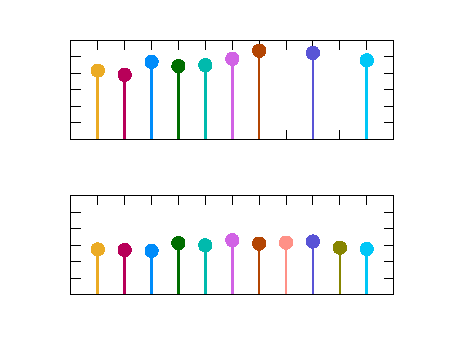
\includegraphics{./figures/parts/02/chapters/03/sections/04/csal_execution_times}}%
    \gplfronttext
  \end{picture}%
\endgroup

    \caption{}
    \label{}
    \end{subfigure}
\caption{}
\label{}
\end{figure}

%%%%%%%%%%%%%%%%%%%%%%%%%%%%%%%%%%%%%%%%%%%%%%%%%%%%%%%%%%%%%%%%%%%%%%%%%%%%%%%%
\subsection{Αξιολόγηση}
\label{subsection:02_03_04:03}

Εξετάζοντας τα στοιχεία \ref{fig:xy_errors_all}-\ref{fig:execution_times_csal}
συνολικά, αυτό που διακρίνεται με την πρώτη ματιά είναι ότι η θέση και ο προσανατολισμός
σφάλματα της PGL-FMIC ήταν ασυσχέτιστα με την ποσότητα του θορύβου που διαταράσσει την
εύρους του φυσικού αισθητήρα LIDAR. Εκείνα του PLICP ήταν ανάλογα ή
αναλλοίωτα σε αυτόν, λόγω της εξαιρετικής απόδοσής του στην εύρεση αντιστοιχιών
μεταξύ των ακτίνων, όποτε αυτό είναι δυνατόν. Όσον αφορά τα μεγέθη τους, δεν υπάρχει σαφής
μοτίβο κυριαρχίας του ενός αλγορίθμου έναντι του άλλου. Για τον PGL-FMIC το μέγιστο
σφάλμα εντοπισμού των ακροβατών ήταν μικρότερο από $0.45$ m σε όλες τις διαμορφώσεις που δοκιμάστηκαν.
Ο χρόνος εκτέλεσής του ήταν περίπου $50\%$ περισσότερος από αυτόν του PLICP για χαμηλό
αριθμό ακτίνων αισθητήρων ($720$), αλλά η σχέση αυτή αντιστρέφεται όταν ο αριθμός των
ακτίνων τριπλασιάζεται σε μέγεθος.

Εξετάζοντας τα αποτελέσματα πιο προσεκτικά αποκαλύπτεται ότι οι απαντήσεις της PGL-FMIC περιλάμβαναν ένα
μικρότερο αριθμό ακραίων λύσεων από εκείνες της PLICP. Στο περιβάλλον CORRIDOR
η πρώτη παρήγαγε μία ακραία λύση σε προσομοιώσεις $3\times4\times100 = 1200$.
Η PLICP απέτυχε περίπου μία φορά κάθε τέσσερις προσπάθειες επίλυσης του προβλήματος όταν
το ρομπότ ήταν τοποθετημένο στο σημείο $\bm{p}_b^C$, μη μπορώντας να διακρίνει μεταξύ του
δύο σχεδόν πανομοιότυπες διακλαδώσεις στο περιβάλλον.

Στο περιβάλλον HOME και οι δύο αλγόριθμοι απέτυχαν να εντοπίσουν το ρομπότ όταν το πραγματικό του
θέση του ήταν $\bm{p}_j^H$ λόγω της επανάληψης του περιβάλλοντός του στο
περιβάλλον και στο χάρτη, και επομένως στην ασάφεια της θέσης του ρομπότ.
περιβάλλοντος του ρομπότ. Το PLICP απέτυχε να εντοπίσει το ρομπότ για δύο επιπλέον στάσεις
($\bm{p}_h^H$ και $\bm{p}_i^H$), και συνολικά παρουσίασε περισσότερες ακραίες τιμές από ό,τι το
PGL-FMIC όσον αφορά και τις έντεκα δοκιμασμένες στάσεις σε αυτό το περιβάλλον. Οι παραπάνω
οδηγούν στο αναμενόμενο συμπέρασμα ότι, όποτε και αν είναι δυνατόν, είναι
καλύτερα να τοποθετείται το ρομπότ σε θέσεις των οποίων το περιβάλλον δεν επαναλαμβάνεται σε
το σύνολο του χάρτη.\footnote{Η τοποθέτηση ενός αποσαφηνιστικού αντικειμένου στο
περιβάλλον πριν από την κατασκευή του χάρτη του θα αύξανε τουλάχιστον την πιθανότητα
της επιτυχούς επίλυσης της ασάφειας της στάσης σε περιβάλλοντα που παρουσιάζουν
επαναλαμβανόμενες δομές}

Στο περιβάλλον WAREHOUSE η ανεπάρκεια της μέγιστης εμβέλειας από το LIDAR του ρομπότ
σε σχέση με τις αποστάσεις μεταξύ των αντικειμένων και τη σπανιότητά τους
είχε ως αποτέλεσμα η PLICP να μην είναι σε θέση να εντοπίσει το ρομπότ σε όλα τα δοκιμασθέντα, εκτός από ένα
στάσεις. Συγκριτικά, η PGL-FMIC επηρεάστηκε λιγότερο από την επίδραση των ελλιπών
πληροφοριών, αδυνατώντας να εντοπίσει το ρομπότ μόνο όταν η θέση του ήταν
$\bm{p}_e^W$. Αυτό οδηγεί στο συμπέρασμα ότι, τουλάχιστον όσον αφορά την PGL-FMIC,
το ρομπότ θα πρέπει να τοποθετείται σε μια θέση που μεγιστοποιεί τον αριθμό της εμβέλειας
μετρήσεων που αναφέρουν τιμές διαφορετικές από εκείνη της μέγιστης εμβέλειας του LIDAR.

Στο περιβάλλον WILLOWGARAGE το PLICP δεν μπόρεσε να εντοπίσει το ρομπότ για τέσσερις από τις
από τις δέκα στάσεις που δοκιμάστηκαν. Για αυτές τις τέσσερις στάσεις μόνο ένας περιορισμένος αριθμός ακτίνων μετέφερε
πληροφορίες που έλειπαν. Ίσως αυτό το αποτέλεσμα, σε συνδυασμό με την εικασία ότι αυτές οι
πρέπει να θεωρηθούν ως ακραίες τιμές από το PLICP--και επομένως ότι οι παράμετροι
που σχετίζονται με την απόρριψη των ακραίων τιμών πρέπει να ρυθμιστούν αναλόγως-- οδήγησε στην
ανεπάρκεια σε αυτό το περιβάλλον. Κατά συνέπεια, εάν εφαρμοστεί η ίδια λογική και
ακολουθηθεί, το ίδιο θα μπορούσε να ειπωθεί και για τις προσομοιώσεις στο περιβάλλον WAREHOUSE,
ωστόσο, ο στόχος μας εδώ είναι να αποφύγουμε τον συντονισμό των παραμέτρων με ad hoc τρόπο ή σε
ανά τοποθεσία ή περιβάλλον, όπως εξηγείται στην ενότητα
\ref{sec:motivation}. Αντιθέτως, η PGL-FMIC δεν μπόρεσε να εντοπίσει το ρομπότ
μόνο σε μία περίπτωση ($\bm{p}_j^G$), για την οποία και οι δύο αλγόριθμοι δεν μπορούσαν να
να επιλύσουν την οκταπλή ασάφεια του περιβάλλοντος χώρου της πραγματικής πόζας. Περιέργως το
ωστόσο, ο PGL-FMIC κατάφερε να επιλύσει την ίδια ασάφεια για τις πόζες $\bm{p}_h^G$
και $\bm{p}_i^G$, ενώ η PLICP ξεπέρασε σημαντικά τον εαυτό της για την πρώτη
αλλά οριακά για τη δεύτερη. Συνολικά η PGL-FMIC κατάφερε να παράγει σωστές
λύσεις για όλες τις περιπτώσεις και να επιλύσει όλες τις ασάφειες πόζας που προκύπτουν από την επανάληψη
του περιβάλλοντος, εκτός από τις περιπτώσεις των $\bm{p}_j^G$ και $\bm{p}_d^G$. Για το
τελευταία, σχεδόν το $50\%$ όλων των λύσεων ήταν λανθασμένες και η PGL-FMIC παρουσίασε περισσότερες
ακραίες τιμές από την PLICP. Η επιπρόσθετη επίλυση ασάφειες διευκολύνθηκε από
μείωση του ανώτερου ορίου κλίμακας $\overline{\sigma}$ από $1.2$ σε $1.1$ στο
στις περιπτώσεις όπου το ρομπότ βρισκόταν σε ασαφές περιβάλλον. PGL-FMIC
παρήγαγε περιορισμένο αριθμό λύσεων με ακραίες τιμές όταν η τυπική κατανομή
του θορύβου που επιδρά στις ακτίνες της πραγματικής σάρωσης τέθηκε στην υψηλότερη τιμή της. Δεδομένου του
τα αποτελέσματα για αυτό το περιβάλλον, όπου η ανάλυση του χάρτη του είναι πιο χονδροειδής
από ό,τι στις τρεις περιπτώσεις που προηγούνται, δεν υπάρχουν στοιχεία που να υποστηρίζουν ότι
η μεταβολή της ανάλυσης επιδεινώνει (ή βελτιώνει) το αποτέλεσμα οποιασδήποτε από τις δύο μεθόδους
που δοκιμάστηκε.

Στο περιβάλλον LANDFILL η PGL-FMIC παρουσίασε λιγότερες ακραίες τιμές από την PLICP, με
διαφορετικές πόζες που προκαλούν κάθε αλγόριθμο: Ο PLICP δεν μπόρεσε να εντοπίσει συνολικά
να εντοπίσει μια πόζα του ρομπότ ($\bm{p}_g^L$), ενώ ο PGL-FMIC εντόπισε με επιτυχία
το ρομπότ περίπου 3 στις 10 φορές όταν αυτό τοποθετήθηκε στη θέση $\bm{p}_f^L$.
Η μη δομημένη φύση του περιβάλλοντος LANDFILL επηρέασε την απόδοση της PGL-FMIC
περισσότερο από τα άλλα (δομημένα) περιβάλλοντα, και περισσότερο όσον αφορά την
απόκριση θέσης και όχι από τα σφάλματα προσανατολισμού του.

Στο πραγματικό περιβάλλον του CSAL AUTh, τα μέσα σφάλματα θέσης και προσανατολισμού δεν
δεν ξεπέρασαν τα $0.35$ m και $0.11$ rad αντίστοιχα για την PGL-FMIC. Η PLICP δεν
κατάφερε να εντοπίσει δύο στάσεις του ρομπότ ($\bm{p}_h^A$ και $\bm{p}_j^A$), για τις οποίες
PGL-FMIC κατάφερε να εντοπίσει το ρομπότ τρεις από τις πέντε φορές. Όσον αφορά
τους χρόνους εκτέλεσης, αυτοί ήταν αυξημένοι και για τις δύο εξεταζόμενες μεθόδους λόγω της
αυξημένου αριθμού ακτίνων του αισθητήρα YDLIDAR σε σύγκριση με τις προσομοιωμένες
φυσικό αισθητήρα (201$ έναντι 720$). Οι χρόνοι της προτεινόμενης μεθόδου ήταν αυξημένοι
περίπου κατά δύο φορές, ενώ οι χρόνοι της PLICP αυξήθηκαν κατά τόσο
τέσσερις φορές. Κατά συνέπεια, συμπεραίνουμε ότι ο χρόνος εκτέλεσης της PGL-FMIC
είναι ανάλογος του αριθμού των ακτίνων του αισθητήρα εμβέλειας, αλλά παρουσιάζει ασθενέστερη
εξάρτηση από αυτές σε σύγκριση με την PLICP.

Συνολικά, όσον αφορά τα κριτήρια για τις λύσεις πόζας, η PGL-FMIC παρουσίασε
σημαντική διαφορά στον αριθμό των λύσεων πόζας που θα ήταν αποδεκτές
στην επακόλουθη εργασία εντοπισμού της στάσης σε σύγκριση με την PLICP. Αποτυχία της PGL-FMIC
όσον αφορά τις αποδεκτές λύσεις οφειλόταν α) στην αποτυχία επίλυσης των
πανομοιότυπων ή παρόμοιων περιβαλλόντων, β) στην έλλειψη πληροφοριών για το εύρος σε ένα
και γ) υπερβολικό θόρυβο από το εύρος. Όσον αφορά την ακρίβεια της
παραδεκτών λύσεων πόζας, δεν υπάρχει σημαντική διαφορά στην ακρίβεια της πόζας
σε σύγκριση με την PLICP. Το τελικό κριτήριο του συνολικού προσδιορισμού της στάσης
με βάση τον βαθμό ομοιότητας που εκδίδεται από το FMI-SPOMF και τα κατώτατα όρια κλίμακας
που χρησιμοποιήθηκαν (υποενότητα \ref{subsec:pose_selection}) ήταν, εντός λογικών ορίων, καλά συμπεριφερόμενα
καθολικοί διαχωρισμοί μεταξύ υποθέσεων.
